\documentclass[a4paper,12pt]{elsarticle}


\usepackage[utf8]{inputenc}
\usepackage[english]{babel}
\usepackage{mathtools}     % it also loads amsmath
\usepackage{amssymb}       % it also loads amsfonts
\usepackage{bm}            % bold Greek letters
\usepackage{xfrac}         % slanted fraction
\usepackage{hyperref}      % requires manual specification of author and title
\usepackage{fix-cm}        % arbitrary font size
\usepackage{array}         % extending tabular environment
\usepackage{subcaption}    % sub-figures
\usepackage{float}         % placing figures
\usepackage{xcolor}

\hypersetup{
    pdftitle={A FIC-FEM procedure for the shallow water equations over partially wet domains},
    pdfauthor={M. Masó, I. de-Pouplana, E. Oñate}
}

\newcommand{\Ignasi}[1]{\textcolor{blue}{#1}}
\newcommand{\Miguel}[1]{\textcolor{red}{#1}}
\newcommand{\pder}[2]{\frac{\partial#1}{\partial#2}}
\newcommand{\ppder}[2]{\frac{\partial^2#1}{\partial#2^2}}
\newcommand{\abs}[1]{\lvert#1\rvert}
\newcommand{\norm}[1]{\lVert#1\rVert}
\newcommand{\defeq}{\mathrel{\vcenter{\baselineskip0.5ex\lineskiplimit0pt\hbox{\scriptsize.}\hbox{\scriptsize.}}}=}


\begin{document}

\hyphenation{Uni-ver-sitat Poli-tec-nica Cata-lunya}

\begin{frontmatter}
\title{A FIC-FEM procedure for the shallow water equations over partially wet domains}
\author[1,2]{Miguel Masó \corref{cor1}}
\ead{mmaso@cimne.upc.edu}
\author[1,2]{Ignasi de-Pouplana}
\author[1,2]{Eugenio Oñate}
\cortext[cor1]{Corresponding author}
\address[1]{Centre Int. de Mètodes Numèrics a l'Enginyeria (CIMNE), Barcelona, Spain}
\address[2]{Universitat Politècnica de Catalunya (UPC), Barcelona, Spain}

\begin{abstract}
We present a stable finite element formulation for the shallow water equations using the finite increment calculus (FIC) procedure.
This research is focused on the stability properties of the FIC technique and uses linear triangles for the spatial discretization with an equal order of interpolation for all the variables.
The extension to higher order polynomial interpolation functions and different geometries is straightforward.
The present FIC-FEM procedure is also able to introduce artificial viscosity for an adequate shock capturing.
An implicit time integration has been used. Special attention has been payed to the dry domain in order to solve the moving boundaries with a fixed mesh eulerian approach.
Three academic examples are included in order to test the capabilities of the FIC-FEM procedure: the global stabilization, the shock capturing technique and the dry-wet interface.
An experimental benchmark tests the overall accuracy of the present formulation.
\end{abstract}

\begin{keyword}
shallow water equations \sep finite element method \sep continuous Galerkin \sep FIC stabilization \sep dry-wetting model
\end{keyword}
\end{frontmatter}


\section{Introduction}


The shallow water equations are often used to study the hydrological dynamics of rivers and estuaries or coastal hydrodynamics.
Derived from the vertical integration of the three-dimensional (3D) Navier-Stokes equations, the shallow water equations define an averaged free surface flow in the horizontal plane.
Due to the complexity of the geometry and the source terms is not possible to find an analytical solution for the PDE's, this explains the need to design strategies to find numerical solutions.
In those physical phenomena, flooding or moving shoreline may occur, which is numerically defined by a null water depth.

The shallow water equations have traditionally been modelled using finite volumes (FV) because of its advantages of stability and monotonicity. Given its geometric flexibility and its natural way to introduce high order schemes, the finite element method (FEM) has been applied too \cite{zien3,navon1979,navon1988}.
% However, since the FEM can exhibit spurious oscillations, different strategies have been proposed; such as the discontinuous Galerkin (DG) technique has been introduced \cite{ambati2007,khan2014,lee2019}.
% DG method has the advantages of the geometrical flexibility of the finite elements and the stability of finite volumes, but the introduction of high order DG schemes is not straightforward.
% In order to prevent numerical instabilities in finite elements, stabilization, monotonic schemes or different order of polynomial interpolation can be explored \cite{hood1974,zien3,ortiz2012}.
However, since the FEM can exhibit spurious oscillations, different strategies such as stabilization, monotonic schemes or different order of polynomial interpolation can be explored \cite{hood1974,zien3,ortiz2012}.
As an alternative to the continuous FEM, more recently the discontinuous Galerkin (DG) technique has been introduced \cite{ambati2007,khan2014,lee2019}.
DG method has the advantages of the geometrical flexibility of the FEM and the stability of FV, but the introduction of high order DG schemes is not straightforward.
This research is focused in classical stabilized finite elements with an equal order interpolation for all the variables. We will explore the capabilities of the finite increment calculus (FIC) technique to develop stable formulations for the shallow water equations.

Several families of stabilization methods can be found in the literature, usually applied to the convection-diffusion equations and the Navier-Stokes equations. The most relevant are SUPG \cite{brooks1982},
ASGS\cite{codina1998}, GLS \cite{hughes1989} and FIC\cite{onate1996,onate1998}.
Due to the hyperbolic character of the shallow water equations, a particular stabilization method for compressible flow or the Euler equations need to be developed.
The FIC approach is based on the incremental solution of a modified system of non-local governing equations accounting for higher order terms obtained by applying the balance laws in domains of finite size.
The FIC-based stabilization has been applied in conjunction with the FEM to convection-diffusion, incompressible flows, among other applications \cite{onate1998,onate2001}.
In those cases, where the convective term has an important role, a first order FIC term is enough to provide stability to the system.
However, the shallow water equations are governed by the convective term and the wave equation in a mixed formulation \cite{codina2008}. In consequence, the common derivation of the FIC-based stabilization is not enough to provide stability in all the range of applicability of the shallow water equations. 
A generalization of this method is proposed in order to provide a global stability for the shallow water equations.

Once global stability is achieved, local instabilities may appear near discontinuities, which are inherent to the supercritical flows.
A local shock capturing technique was initially proposed by Hughes \cite{hughes1986} and a review of shock capturing techniques can be found in Codina \cite{codina2011}.
Other possibilities of the FIC-based formulations are explored to provide a shock capturing stabilization \cite{cotela2016}.

Additionally, the dry domain requires an accurate modeling because the hyperbolic equations require positive water depth in all the domain.
Several authors have proposed different methods to solve the shallow water equations with moving shoreline. Leclerc et al. \cite{leclerc1990} proposed an Eulerian method. Later, Heniche et al. \cite{heniche2000} modified the method allowing the free surface to plunge under the topography.
Other authors developed a rough-porous layer \cite{candy2017,barros2011} or a modified depth integration \cite{defina2000}. These approaches introduce new physical parameters in the balance equations.
An Eulerian approach based on the work of \cite{leclerc1990} and \cite{heniche2000} is presented.


This article is organized as follows. Firstly the governing equations of the shallow water problems are presented.
In Section \ref{sec:stabilization} the FIC stabilization procedure is applied to add the stabilization terms and the shock capturing terms.
In Section \ref{sec:fem} the spatial (FEM) and temporal discretizations are described.
The dry domain model is presented in the same section because it mainly depends on the discretization.
Section \ref{sec:examples} presents some numerical examples.
The first simple example tests the stability, the second one tests the shock capturing and the third one tests the dry-wet interface.
The last example is a simulation of an experiment and the results are compared with the reference.
The conclusions are given in Section \ref{sec:conclusions}.


\section{Governing equations and linearization}

The shallow water equations are the result of integrating vertically the Navier-Stokes equations, assuming the vertical velocity and its acceleration negligible \cite{abbot1979,zien3}.
The equations governing mass and momentum conservation can be written in conservative form with water depth $h$ and specific discharge $\mathbf{q}=(h\mathbf{u})$ as follows,

\begin{equation} \label{general_sw}
\pder{\bm{\phi}}{t} + \pder{\mathbf{F}_i}{x_i} + \pder{\mathbf{G}_i}{x_i} + \mathbf{Q} = \mathbf{0} \quad \text{for} \enspace i=1,2
\end{equation}
with

\begin{subequations}\label{variables_and_fluxes}
\allowdisplaybreaks
\begin{align}
\bm{\phi} &= \left\{
    \begin{array}{c}
        hu_1 \\
        hu_2 \\
        h
    \end{array}\right\} \\
\mathbf{F}_i &= \left\{
    \begin{array}{c}
        hu_1u_i + \delta_{1i}\frac{1}{2}g(h^2 - z^2) \\ [5pt]
        hu_2u_i + \delta_{2i}\frac{1}{2}g(h^2 - z^2) \\ [5pt]
        hu_i
    \end{array}\right\} \\
\mathbf{G}_i &= \left\{
    \begin{array}{c}
        -(h/\rho) \bar{\tau}_{1i} \\ [5pt]
        -(h/\rho) \bar{\tau}_{2i} \\ [5pt]
        0
    \end{array}\right\} \\
\mathbf{Q} &= \left\{
    \begin{array}{c}
        \displaystyle -g(h-z)\pder{z}{x_1} + \frac{h}{\rho}\pder{p_a}{x_1}
        - \frac{1}{\rho}\tau^s_{31} + \frac{1}{\rho}\tau^b_{31} \\ [10pt]
        \displaystyle -g(h-z)\pder{z}{x_2} + \frac{h}{\rho}\pder{p_a}{x_2}
        - \frac{1}{\rho}\tau^s_{32} + \frac{1}{\rho}\tau^b_{32} \\ [10pt]
        r
    \end{array}\right\}
\end{align}
\end{subequations}
where $\bm{\phi}$ is the vector of conserved variables, $\mathbf{F}_i$ is the vector of convective fluxes, $\mathbf{G}_i$ is the vector of viscous fluxes and $\mathbf{Q}$ is the vector source terms. In Figure \ref{diagram} there is a representation of the variables and the notation. The coordinates are denoted with the index notation $x_i$, with $i=1,3$, while the number of dimensions $n_d$ is equal to 2. $\delta_{ij}$ is the Kronecker delta. The topography is expressed with the variable $z$ and the free surface elevation is expressed in terms of the topography and the total depth, $\eta = z + h$. $\bar{\tau}_{ij}$ are the averaged horizontal stresses, and $\tau^b_{3i}$ and $\tau^s_{3i}$ denote the bottom and surface friction stresses respectively. Finally, $r$ is the rain source term and $p_a$ is the atmospheric pressure.

\begin{figure}
    \centering
    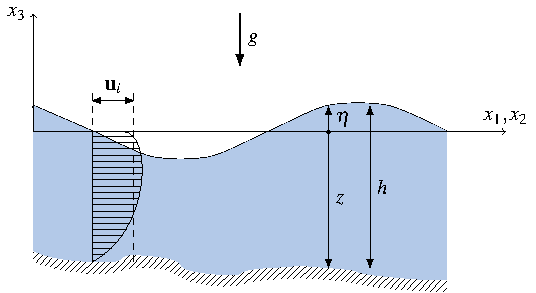
\includegraphics[width=.8\textwidth]{img/fig/diagram.pdf}
    \caption{Diagram and notation for the balance equations (\ref{general_sw}) and (\ref{variables_and_fluxes})}
    \label{diagram}
\end{figure}

The problem is closed with an initial boundary condition,

\begin{equation}
\bm{\phi}(t=t_0) = \bm{\phi}_0
\end{equation}
where $\bm{\phi}_0$ are the initial water height and specific discharge. Equation (\ref{general_sw}) satisfy the standard boundary conditions in space

\begin{align}
\bm{\phi} = \bm{\phi}_D \qquad &\text{in} \ \Gamma_D \\
\mathbf{F}_i\mathbf{n} = F_N \qquad &\text{in} \ \Gamma_N
\end{align}
where $\Gamma_D$ represents the part of the Dirichlet boundary conditions and $\Gamma_N$ represents the part of the Neumann boundary conditions. We will consider absorbing boundary conditions ind $\Gamma_A$, such that $\Gamma_D \cap \Gamma_N \cap \Gamma_A = \delta\bm{\Omega}$.

The bottom friction $\tau^b_{3i}$ is modelled with the Manning formula generalized for two dimensions as

\begin{equation}
\frac{\tau^b_{3i}}{\rho} = -gn^2\frac{\abs{\mathbf{u}}\mathbf{u}}{h^{\sfrac{4}{3}}}
\end{equation}

The averaged horizontal stresses are calculated from the combination of the molecular stresses and the Reynolds stresses as follows

\begin{equation} \label{stresses}
\frac{\tau_{ij}}{\rho} = (\nu + \nu_t)\left(
    \pder{u_i}{x_j} + \pder{u_j}{x_i} -\frac{2}{3}\delta_{ij}\pder{u_k}{x_k} \right)
\end{equation}

The balance equation (\ref{general_sw}) is linearized in the following form

\begin{equation}
\pder{\bm{\phi}}{t} + \mathbf{A}_i\pder{\bm{\phi}}{x_i}
 - \pder{}{x_k}\left(\mathbf{K}_{ik}\pder{\bm{\phi}}{x_i}\right) + \mathbf{S}\bm{\phi} + \mathbf{T} = 0
\end{equation}
where the matrices $\mathbf{A}_i$ and $\mathbf{K}_{ik}$ are the linearization matrices of the convective fluxes and the diffusive fluxes respectively. The convective matrices $\mathbf{A}_i$ are obtained after applying the chain rule to the vector of fluxes $\mathbf{F}_i$,
\begin{subequations}
\begin{align}
\pder{\mathbf{F}_i}{x_i} &= \pder{\mathbf{F}_i}{\bm{\phi}}\pder{\bm{\phi}}{x_i} \\
\mathbf{A}_i &= \pder{\mathbf{F}_i}{\bm{\phi}}
\end{align}
\begin{equation}
\mathbf{A}_1 = \left[\begin{matrix}
        2u_1 & 0   & -u_1^2 + c^2 \\
        u_2  & u_1 & -u_1 u_2 \\
        1    & 0   & 0
    \end{matrix} \right]
\quad , \quad
\mathbf{A}_2 = \left[\begin{matrix}
        u_1 & u_2  & -u_1 u_2 \\
        0   & 2u_2 & -u_2^2 + c^2 \\
        1   & 0    & 0
    \end{matrix} \right]
\end{equation}
\end{subequations}
and $c=\sqrt{gh}$ is the wave speed. The matrices $\mathbf{A}_i$ define an hyperbolic ODE and its eigenvalues are $u+c$, $u$ and $u-c$, which requires positivity of the water column depth $h$.

The bottom friction term is linearized using a reaction matrix $\mathbf{S}$
\begin{equation}
\mathbf{S} = \left[\begin{matrix}
    \frac{g\abs{\mathbf{u}}}{n^2h^{4/3}} & 0 & 0 \\
    0 & \frac{g\abs{\mathbf{u}}}{n^2h^{4/3}} & 0 \\
    0 & 0 & 0
\end{matrix}\right]
\end{equation}
In the following sections, the rain, the atmospheric pressure gradient and the wind friction will be neglected, retaining the topography gradient in the source vector $\mathbf{T}$.

\section{FIC stabilization}\label{sec:stabilization}

We will consider the quasi-linear balance equations written in residual form as a vector

\begin{equation} \label{residual}
\mathbf{r} \defeq 
  \pder{\bm{\phi}}{t} + \mathbf{A}_i\pder{\bm{\phi}}{x_i}
  -\pder{}{x_k}\left(\mathbf{K}_{ik}\pder{\bm{\phi}}{x_i}\right) + \mathbf{S}\bm{\phi} + \mathbf{T} \qquad i,k\in\{1,n_d\}
\end{equation}
where $n_d=2$ is the number of dimensions. The size of the vector $\mathbf{r}$ is equal to the number of balance equations, $n_b=3$.

In the one dimensional case ($n_d=1$) and scalar balance ($n_b=1$), the FIC-based stabilization is based on a modified non local version of the governing equations as \cite{onate1998}

\begin{equation}
r - \frac{1}{2}l^e\pder{r}{x} = 0
\end{equation}

The stabilization parameter $l^e$ is usually taken the element length. However, in 2D and 3D, or when the number of balance equations $n_b$ is different than $n_d$, the choice of the $l^e$ parameter is non trivial.
Several approaches can be found in the literature. In \cite{onate1998} $l^e$ is chosen as a vector, but in later publications such as \cite{onate2001} a generalized formulation for different values of $n_d$ and $n_b$ was presented.
For the stabilization of the Navier-Stokes equations different projections of the element size over the velocity and over the velocity gradient have been proposed \cite{cotela2016}. Here we will use index notation for the residual vector $\mathbf{r}$ in order to distinguish the indices that goes to $n_d$ or to $n_b$. To sum up, the different forms of the FIC stabilization procedure can be written as

\begin{subequations}
\begin{align}
r_j - \frac{1}{2}l^e_i\pder{r_j}{x_i} &= 0
    \qquad i\in\{1,n_d\} \ ,\ j\in\{1,n_b\}\\[5pt]
r_j - \frac{1}{2}l^e_u\frac{u_i}{\norm{\mathbf{u}}}\pder{r_j}{x_i} &= 0
    \qquad i,j\in\{1,n_d\}\\[5pt]
r_j - \frac{1}{2}l^e_{g_i}\frac{\sfrac{\partial\mathbf{u}}{\partial x_i}}{\norm{\nabla u_i}}\pder{r_j}{x_i} &= 0
    \qquad i,j\in\{1,n_d\}
\end{align}
\end{subequations}

%The FIC stabilization has been applied to problems with one balance equation (see \cite{onate1998} for the stabilization of the convection diffusion problem) or problems where the number of balance equations coincide with the number of space dimensions ($n_d = n_b$) (see \cite{onate1998} for the stabilization of the momentum and pressure equations of the Navier-Stokes equations).
In this paper we propose a stabilization term which is oriented along the characteristics of the hyperbolic equations, as

\begin{equation} \label{fic_sw}
r_j - \frac{1}{2}l^e\frac{\mathbf{A}_i}{\lambda}\pder{r_j}{x_i} = 0
    \qquad i\in\{1,n_d\} \ ,\ j\in\{1,n_b\}
\end{equation}
For consistency the linearization matrix $\mathbf{A}_i$ is normalized with the maximum eigenvalue $\lambda$. This stabilization is analogue to the virtual multi-scale stabilization proposed in \cite{codina2008b}. The linearization matrix $\mathbf{A}_i$ provides a weighting procedure between the stabilization of the convective and the mixed wave equation terms. In practice the element size is multiplied by an algorithmic constant in order to control the amount of diffusion added by the stabilization and it will be studied in the examples of Section \ref{sec:examples}. Recovering the vector notation for the residual, the FIC-balance reads
\begin{equation} \label{fic_sw_beta}
\mathbf{r} - \beta l^e\frac{\mathbf{A}_i}{\lambda}\pder{\mathbf{r}}{x_i}
    \qquad i\in\{1,n_d\}
\end{equation}

The FIC formulation is the result of introducing the residual of the shallow water equations (\ref{residual}) into the expression in Eq (\ref{fic_sw_beta}). The variational expression of the equation is obtained by multiplying the equation by a test function $\omega_k$ and integrating over the domain $\Omega$. This gives

\begin{equation} \label{variational_fic}
\int_\Omega \left(
    \omega_k \mathbf{r} + \omega_k \beta l^e\frac{\mathbf{A}_i}{\lambda}\pder{\mathbf{r}}{x_i}
\right) d\Omega = 0
\end{equation}
The second term of Equation (\ref{variational_fic}) is integrated by parts. Note that the element length $l^e$, the linearization matrix $\mathbf{A}_i$ and its eigenvalue $\lambda$ are defined constant inside the element. Hence, the boundary integral which appears after integration by parts should be understood as the boundary of all the elements

\begin{equation} \label{variational_fic_parts}
\int_\Omega \omega_k \mathbf{r} d\Omega
+ \int_\Omega \beta l^e\frac{\mathbf{A}_i}{\lambda}\pder{\omega_k}{x_i} \mathbf{r} d\Omega
+ \sum_e \int_{\Gamma_e} \beta l^e\frac{\mathbf{A}_i}{\lambda}\omega_kn_k \mathbf{r} d\Gamma = 0
\end{equation}
In this work we neglect the boundary integrals assuming that the residual $\mathbf{r}$ is null at the boundary of the elements. At this point we introduce the balance Equation (\ref{residual}) and integrate by parts the diffusive term. The result is

\begin{multline} \label{variational_balance_fic}
\int_\Omega \left(
    \omega_k \pder{\bm{\phi}}{t} + \omega_k \mathbf{A}_i\pder{\bm{\phi}}{x_i}
    + \pder{\omega_k}{x_j} \mathbf{K}_{jk} \pder{\bm{\phi}}{x_i} + \mathbf{S}\bm{\phi} + \mathbf{F}
\right) d\Omega\\ +
\int_\Omega \frac{\beta l^e}{\lambda} \left(
    \pder{\omega_k}{x_j} \mathbf{A}_j \pder{\bm{\phi}}{t}
    + \pder{\omega_k}{x_j} \mathbf{A}_j\mathbf{A}_i\pder{\bm{\phi}}{x_i}
    + \ppder{\omega_k}{x_j} \mathbf{A}_j\mathbf{K}_{jk} \pder{\bm{\phi}}{x_i} \right. \\
    \left.
    + \pder{\omega_k}{x_j} \mathbf{A}_j(\mathbf{S}\bm{\phi} + \mathbf{F})
\right) d\Omega
=0
\end{multline}
Equation (\ref{variational_balance_fic}) is the stabilized variational form for the shallow water equations, similar to the expression obtained by SUPG. Note that the parameter $\beta l^e/\lambda$ is analogous to the characteristic time $\tau$ of the classical SUPG or GLS techniques \cite{cotela2016}.

\subsection{Shock capturing stabilization}

In this section we explore other possibilities of the characteristic length definition in order to obtain a shock capturing stabilization. Here, the mass balance and the momentum balance are considered separately and the characteristic length is projected onto the gradient of the unknown

\begin{subequations} \label{eq:shock_capt}
\begin{align}
\text{Momentum balance:} &&
    r_i^q + \frac{l^e}{2\norm{\nabla q_i}}\pder{q_i}{x_j}\pder{r_i^q}{x_j} &= 0 \label{eq:shock_capt_a} && \\ 
\text{Mass balance:} &&
    r^h + \frac{l^e}{2\norm{\nabla h}} \pder{h}{x_j} \pder{r^h}{x_j} &=0 \label{eq:shock_capt_b}
\end{align}
\end{subequations}

Multiplying the momentum balance Equation (\ref{eq:shock_capt_a}) by a proper test function $\omega_k$ , integrating over the domain in the same way as in Equation (\ref{variational_fic}), and then integrating by parts, one obtains the following variational form:
\begin{equation}
    \int_\Omega \omega_k r_i^q d\Omega
     - \int_\Omega \omega_k \frac{l^e}{2\norm{\nabla q_i}}\pder{q_i}{x_j}\pder{r_i^q}{x_j}
     d\Omega = 0
    \label{partial_variational_shock_capt}
\end{equation}

After integration of Equation (\ref{partial_variational_shock_capt}) by parts and rearranging terms we obtain
\begin{multline}
    \int_\Omega \omega_k r_i^q d\Omega 
    + \int_\Omega \pder{\omega_k}{x_j}
        \frac{l^e r_i^q}{2\norm{\nabla q_i}}\pder{q_i}{x_j} d\Omega \\
    + \int_\Omega \omega_k \pder{}{x_j}\left(
         \frac{l^e}{2\norm{\nabla q_i}}\pder{q_i}{x_j}
        \right)r_i^q d\Omega 
    - \int_\Omega \pder{}{x_j}\left(
        \omega_k \frac{l^e}{2\norm{\nabla q_i}}\pder{q_i}{x_j}r_i^q \right) d\Omega
        = 0
        \label{variational_shock_capturing}
\end{multline}
The last two terms of Equation (\ref{variational_shock_capturing}) are dropped because they involve derivatives of the characteristic length and can be transformed into a boundary integral.

The same procedure is applied to the mass balance equation (\ref{eq:shock_capt_b}). As a result we obtain the following system of equations for both unknowns
\begin{subequations} \label{fic_shock_capturing}
\begin{align}
\text{Momentum balance:} &&
\int_\Omega \omega_k r_i^q d\Omega 
+ \int_\Omega \pder{\omega_k}{x_j}
\frac{l^e r_i^q}{2\norm{\nabla q_i}}\pder{q_i}{x_j} d\Omega &=0 && \\
\text{Mass balance:} &&
\int_\Omega \omega_k r^h d\Omega 
+ \int_\Omega \pder{\omega_k}{x_j}
    \frac{l^e r^h}{2\norm{\nabla h_i}}\pder{q_i}{x_j} d\Omega &=0
\end{align}
\end{subequations}

The above expressions (\ref{fic_shock_capturing}) are equivalent to a classical shock capturing method, in which the artificial diffusivity $k_{art}$ and artificial viscosity $\nu_{art}$ can be identified as
\begin{subequations} \label{k_art}
\begin{equation}
\nu_{art} = \frac{1}{2}\alpha l_e \frac{\abs{R(u_i)}}{\abs{\nabla u_i}}
\end{equation}
\begin{equation}
k_{art} = \frac{1}{2}\alpha l_e \frac{\abs{R(h)}}{\abs{\nabla h}}
\end{equation}
\end{subequations}
where $\alpha$ is an algorithmic constant.

Such approach can be refined by introducing the stabilization along the streamlines. This way, $k_{art}$ and $\nu_{art}$ need to be added only in the crosswind direction. The diffusive term is added to the mass balance with the following orthogonal tensor

\begin{equation}
\mathbf{D}_{art} = k_{art}
\left( \mathbf{I} - \frac{1}{\abs{\mathbf{u}}^2} \mathbf{u} \otimes \mathbf{u} \right)
\end{equation}
The viscosity is introduced into the momentum balance with a fourth order tensor in the crosswind direction. Using Voigt's notation,
\begin{equation}
\mathbf{C}_{art} = \nu_{art} \mathbf{I}_4 \mathbf{J}
\end{equation}
with
\begin{equation}
\mathbf{J} = \left[\begin{matrix}
    1-\frac{q_1q_1}{\mathbf{q}\mathbf{q}} & -\frac{q_1q_2}{\mathbf{q}\mathbf{q}} & 0 \\
    -\frac{q_1q_2}{\mathbf{q}\mathbf{q}} & 1-\frac{q_2q_2}{\mathbf{q}\mathbf{q}} & 0 \\
    0 & 0 & 1-\frac{q_1q_2}{\mathbf{q}\mathbf{q}}
\end{matrix}\right]
\end{equation}
where $\mathbf{I}_4$ is the fourth order identity tensor for the stresses, which is derived from Equation (\ref{stresses}) and will be defined in Section \ref{sec:fem}.

\section{Finite element formulation} \label{sec:fem} 

It is conventional to use higher order of interpolation for the momentum or velocity than for the water depth or free surface in order to develop stable finite element formulations \cite{hood1974,heniche2000,bercovier1979}. In this work we restrict ourselves to linear triangles for both $\mathbf{q}$ and $h$ unknowns, since the FIC-FEM procedure is intrinsically stable. For that reason, all terms including spatial derivatives of order higher than two will be neglected. Bilinear quadrilaterals and higher order elements with the same number of degrees of freedom for all the variables will be also stable.

\subsection{Spatial discretization}

A finite element discretization $\Omega_h$ is introduced in the domain $\Omega$ and the problem variables can be interpolated with the basis functions of the finite elements space as

\begin{equation}
\phi_i = \sum_a^{N_\Omega} N_a(\mathbf{x})\phi_{ai} \qquad i \in \{1,n_b\}
\end{equation}
where $N_\Omega$ represents the total number of nodes in $\Omega_h$ and $\phi_i$ are the problem variables defined in (\ref{variables_and_fluxes}). Here we introduce the notation $\bm{\phi}_h$ for the vectors of nodal unknowns -momentum and water height- on the finite element domain. Following the standard Galerkin discretization, the shape functions $N_a$ are used to interpolate the test functions $\omega_k$ and the unknowns. The continuous equation (\ref{variational_balance_fic}) is combined with equation (\ref{fic_shock_capturing}) and can be expressed as the following algebraic system of equations
\begin{equation} \label{discrete_sw}
[\mathbf{M} + \mathbf{M}_F] \dot{\bm{\phi}}_h
+ [\mathbf{G} + \mathbf{G}_F + \mathbf{L} + \mathbf{L}_{SC} + \mathbf{R} + \mathbf{R}_F] \bm{\phi}_h
= \mathbf{T} + \mathbf{T}_F
\end{equation}
where the dot ($\dot{\ }$) means temporal derivative. The matrices in Eq. (\ref{discrete_sw}) without subscript are related to the original problem (\ref{residual}); the matrices with subscript F correspond to the terms added by the FIC procedure to ensure stability, and those with the subscript SC are the terms added by the shock capturing technique. Using $a$, $b$ to denote the nodes, $i$, $j$ to denote the space dimension index and $k$, $l$ to denote the balance equation number, the matrices in Eq. (\ref{discrete_sw}) are defined as

\begin{align}
    \displaystyle \mathbf{M}^{ab} &= \int_{\Omega_e}N_a \mathbf{I} N_b d\Omega &
    \displaystyle \mathbf{G}^{ab} &= \int_{\Omega_e}
        N_a \mathbf{A}_i \pder{N_b}{x_i} d\Omega \nonumber\\[5pt]
    \displaystyle \mathbf{L}^{ab} &= \int_{\Omega_e}
        \mathbf{B}_a \left[\begin{matrix}
            \mathbf{C} & \mathbf{0} \\ \mathbf{0} & \mathbf{D}
        \end{matrix}\right] \mathbf{B}_b^T d\Omega &
    \displaystyle \mathbf{R}^{ab} &= \int_{\Omega_e} N_a \mathbf{S} N_b d\Omega \\[5pt]
    \displaystyle \mathbf{T}^{ab} &= \int_{\Omega_e} N_a gh\mathbf{z}_b d\Omega +
        \int_{\Gamma_e} N_a \mathbf{t}_b d\Gamma \nonumber
\end{align}
where the diffusive matrix $\mathbf{L}^{ab}$ is defined using the derivatives matrix $\mathbf{B}_a$ and the isotropic tensors $\mathbf{C}$ and $\mathbf{D}$ are given by

\begin{subequations}
\begin{equation}
\mathbf{B}_a = \left[\begin{matrix}
    \pder{N_a}{x_1} & 0 & \pder{N_a}{x_2} & 0 & 0 \\
    0 & \pder{N_a}{x_2} & \pder{N_a}{x_1} & 0 & 0 \\
    0 & 0 & 0 & \pder{N_a}{x_1} & \pder{N_a}{x_2}
\end{matrix}\right]
\end{equation}
\begin{equation}
\mathbf{C} = \nu \mathbf{I}_4 \ , \quad
\mathbf{D} = k \mathbf{I}_2 \ , \quad
\mathbf{I}_4 = \frac{1}{3} \left[\begin{matrix}
        2 & -1 & 0 \\
        -1 & 2 & 0 \\
        0 & 0 & 3
    \end{matrix}\right] \ , \quad
\mathbf{I}_2 = \left[\begin{matrix}
        1 & 0 \\
        0 & 1
    \end{matrix}\right]
\end{equation}
\end{subequations}

The stabilization and shock capturing terms from Equation (\ref{discrete_sw}) result in analogous matrices with higher derivatives order, the boundary integral is neglected, i. e.,

\begin{align}
\displaystyle\mathbf{M}_F^{ab} &= \int_{\Omega_e} \frac{\beta l^e}{2} \pder{N_a}{x_i}\mathbf{A}_i N_b d\Omega &
\displaystyle\mathbf{G}_F^{ab} &= \int_{\Omega_e} \frac{\beta l^e}{2} \pder{N_a}{x_i}\mathbf{A}_i\mathbf{A}_j \pder{N_b}{x_j} d\Omega \nonumber\\
\displaystyle\mathbf{L}_{SC}^{ab} &= \int_{\Omega_e} \frac{\beta l^e}{2} \mathbf{B}_a \left[\begin{matrix}
        \mathbf{C}_\text{art} & \mathbf{0} \\ \mathbf{0} & \mathbf{D}_\text{art}
    \end{matrix}\right] \mathbf{B}_b^T d\Omega &
\displaystyle\mathbf{R}_F^{ab} &= \int_{\Omega_e} \frac{\beta l^e}{2} \pder{N_a}{x_i}\mathbf{A}_i \mathbf{S} N_b d\Omega \\
\displaystyle\mathbf{T}_F^{ab} &= \int_{\Omega_e} \frac{\beta l^e}{2} \pder{N_a}{x_i}\mathbf{A}_i gh\mathbf{x}_b d\Omega
\nonumber
\end{align}


\subsection{Temporal integration}

The resulting expression from the spatial discretization (\ref{discrete_sw}) can be written in the following compact form 
\begin{equation} \label{discrete_compact}
\tilde{\mathbf{M}}\dot{\bm{\phi}}_h + \tilde{\mathbf{K}}\bm{\phi}_h = \tilde{\mathbf{F}}
\end{equation}
where the symbol ($\,\tilde{}\,$) denotes the assembly of the system matrices for all the elements.
We have integrated this equation introducing a time discretization using the well known BDF2 implicit scheme \cite{curtiss1952,brayton1972}. The system of equations in a discrete time domain yields
\begin{equation}
\begin{split} \label{discrete_bdf2}
\tilde{\mathbf{M}}\dot{\bm{\phi}}_h^{n+1} + \tilde{\mathbf{K}}^{n+1}\bm{\phi}_h^{n+1} = \tilde{\mathbf{F}}^{n+1} \\
\dot{\bm{\phi}}_h^{n+1} = \beta_0 \bm{\phi}_h^{n+1} + \beta_1 \bm{\phi}_h^n + \beta_2 \bm{\phi}_h^{n-1}
\end{split}
\end{equation}
We will consider a variable time step to compute the BDF coefficients using the notation $t^{n+1} = t^n + \Delta t^n$:
\begin{equation}
\begin{split}
\beta_0 &= \tau (\rho^2 + 2\rho) \\
\beta_1 &= -\tau (\rho^2 + 2\rho + 1) \\
\beta_2 &= \tau
\end{split}
\end{equation}
with
\begin{equation}
\begin{split}
\tau &= \frac{1}{\Delta t^n(\rho^2 + \rho)} \\
\rho &= \frac{\Delta t^{n-1}}{\Delta t^n}
\end{split}
\end{equation}

The solution of this implicit system requires an iterative procedure. We have used the Newton-Raphson method, by which the problem unknowns are computed in an incremental way as
$\bm{\phi}_h^{n+1,i+1} = \bm{\phi}_h^{n+1,i} + \delta\bm{\phi}_h^i$,
where the superscript $i$ denotes the non linear iteration.
This notation allows us to rewrite the system of equations (\ref{discrete_bdf2}) defining a left hand side matrix multiplied by the increment $\delta\bm{\phi}_h^i$ and a right hand side vector which depends on the previous non linear iteration as
\begin{equation}
[\beta_0\tilde{\mathbf{M}} + \tilde{\mathbf{K}}^{n+1,i}] \delta\bm{\phi}_h^i
= \tilde{\mathbf{F}}^{n+1,i} - \tilde{\mathbf{K}}^{n+1,i}\bm{\phi}_h^{n+1,i} - \tilde{\mathbf{M}}\dot{\bm{\phi}}_h^{n+1,i}
\end{equation}
The first non linear iteration $\bm{\phi}_h^{n+1,0}$ is initialized using a prediction given from the BDF formula at the last time step:
\begin{equation}
\bm{\phi}_h^{n+1,0} = \bm{\phi}_h^n + \Delta t^n \dot{\bm{\phi}}_h^{n}
\end{equation}


\subsection{Dry domain model}

When small or quasi zero water depths are involved in simulations, some instabilities may arise. In addition, the solution of the previous time integration scheme requires the inverse of a matrix which is singular in the dry regions. In this section we review the challenges associated to such a problem, and the way we have circumvented them.

\paragraph{Recovery of the velocity field}
The first issue is the computation of the velocity field, since it involves the division of the discharge by the water height and this operation is ill-conditioned in the dry regions. In this research, the velocity field is computed in a two step procedure. First of all, the velocity is computed at each element following the next expression, initially proposed by Kurganov \cite{kurganov2007}:

\begin{equation} \label{h_inv_kurganov}
h^{-1}_k = \frac{\sqrt{2}\max(h,0)}{\sqrt{h^4 + \max(h^4, \varepsilon^4)}}
\end{equation}
where $\varepsilon$ is a threshold which depends on the elements size; usually $\varepsilon = 0.1 l_e$ is chosen. Figure \ref{inverse_heihgt} shows a dimensionless representation of equation (\ref{h_inv_kurganov}). The second step in the velocity computation is a diffusive projection on the nodes:

\begin{equation}
\mathbf{M}_L \mathbf{u} = h^{-1}_k \mathbf{M} (h\mathbf{u})
\end{equation}
where $\mathbf{M}$ is the consistent mass matrix and $\mathbf{M}_L$ is the lumped mass matrix. This projection will introduce some artificial diffusion in the velocity field near the dry-wet interface reducing the possible maxima extrema.
Additionally, the expression(\ref{h_inv_kurganov}) tends to zero when the water height becomes small, while the analytical expression of the height inverse is recovered when $h>\varepsilon$.


\paragraph{Partially wet elements}
At the elements where the shoreline is located, the interpolated water depth will not represent the real water surface.
Therefore, those elements need an special consideration in order to prevent unrealistic oscillations. Excluding those elements from the computations is equivalent to introduce an artificial barrier, and the inclusion of those elements will incur in a consideration of an extra volume of water.
We chose to include all the elements in the computation and to modify the balance equations in order to satisfy equilibrium at rest (Figure \ref{partially_dry}). This is achieved by introducing a modified topography and imposing equilibrium as
\begin{equation}
    \pder{\eta'}{x_i} = \pder{z'}{x_i} + \pder{h}{x_i} = \mathbf{0}
\end{equation}

\begin{figure}
    \centering
    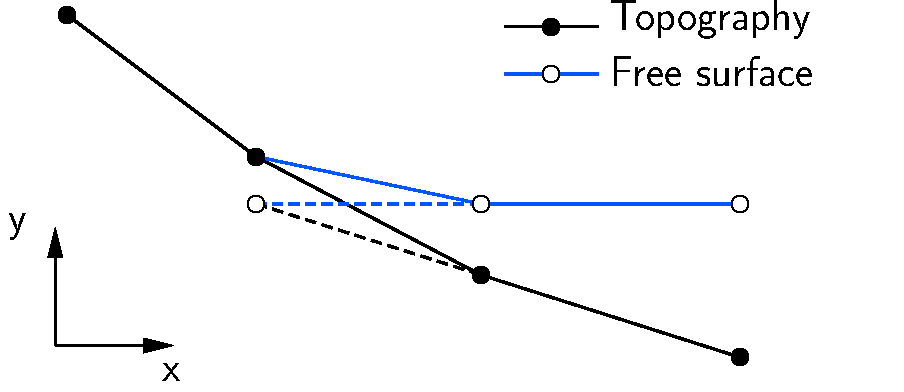
\includegraphics[width=.5\textwidth]{img/fig/partially_dry.pdf}
    \caption{Dry, wet and partially wet elements in 1D. The dashed line shows the modified topography  and the corresponding free surface.}
    \label{partially_dry}
\end{figure}

\paragraph{Avoiding the singularity of the system matrix}
Since all the elements are included in the computational domain, the last issue to overcome with small water depths is the singularity of the system matrix. The mass balance is satisfied in the dry state, but the momentum equation will become unstable. The easiest (although not the most accurate) way to develop a stable scheme is to add a diagonal of non zero terms to the momentum equation, i. e.,

\begin{equation}
\mathbf{G} \defeq \mathbf{G} + \xi\,\text{diag}(1, 1, 0)
\end{equation}

The selection of the areas where there is a dry domain is controlled with a wet fraction function, depicted in Figure \ref{inverse_heihgt}. Expression (\ref{h_inv_kurganov}) allows us to define a wet fraction $\omega$ as
\begin{equation}
\omega = hh^{-1}_k
\end{equation}
and so $\xi$ is defined as
\begin{equation}
\xi = k(1-\omega)
\end{equation}
In our numerical experiments we have chosen $k=10^3$.


\begin{figure}
    \centering
    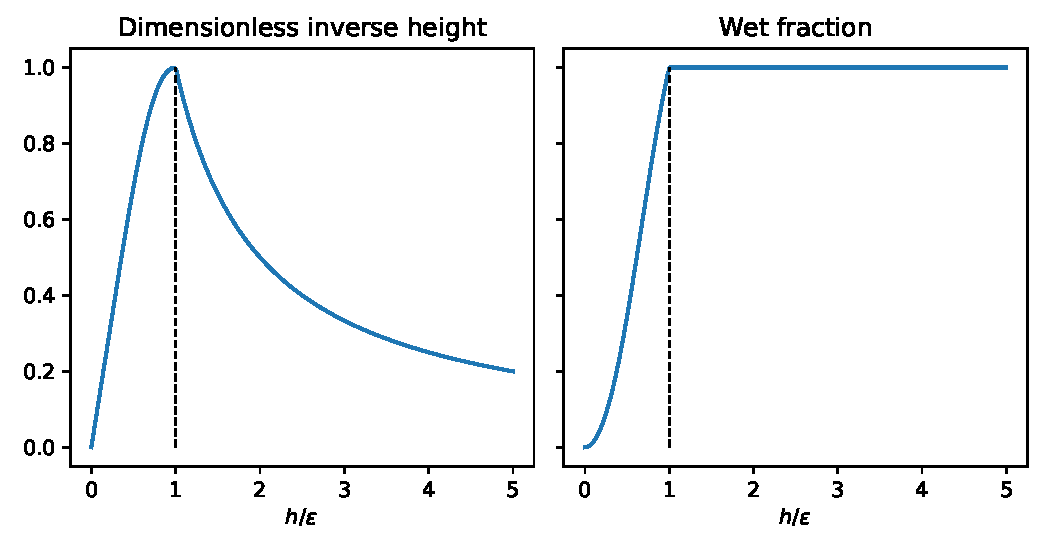
\includegraphics[width=\textwidth]{img/fig/inverse_height.pdf}
    \caption{Dimensionless functions to compute the  inverse height and the wet fraction.}
    \label{inverse_heihgt}
\end{figure}


\section{Examples} \label{sec:examples}

The FIC-FEM formulation presented has been implemented in KratosMultiphysics \cite{dadvand2010, dadvand2013}, an open source framework of numerical methods written in C++.
In this section we present four different examples. Three of them are oriented to verify a single aspect of the procedure explained in this research, the global stabilization, the shock capturing technique and the dry-wet interface.
The last one is devoted to test all the capabilities of the formulation in a practical case for which experimental data is available.


\subsection{Wave in a channel with a backward step}

The aim of the first example is to show that the Galerkin formulation applied to the shallow water equations is unstable and how the present stabilization method can overcome this issue. A calibration of the stabilization parameter is performed to optimize the effect of the stabilization terms in the obtained solution.
We study the propagation of a wave in a channel with a backward step. The wave is reflected at the end and faces the step in the opposite direction. Figure \ref{waves_propagation} shows the propagation of the wave along the channel.
The problem is discretized with a mesh fine enough to test the artificial diffusion added by the stabilization (Figure \ref{step_mesh}). The average element size is $0.06m$ and near the corner the mesh is refined to $0.02m$.
The time step is set automatically to keep a Courant number equal to $1.0$ at every step. The problem is run three times with different algorithmic constants $\beta = 0.001$, $0.01$ and $0.1$. In this example, the shock capturing term is disabled.

\begin{figure}
    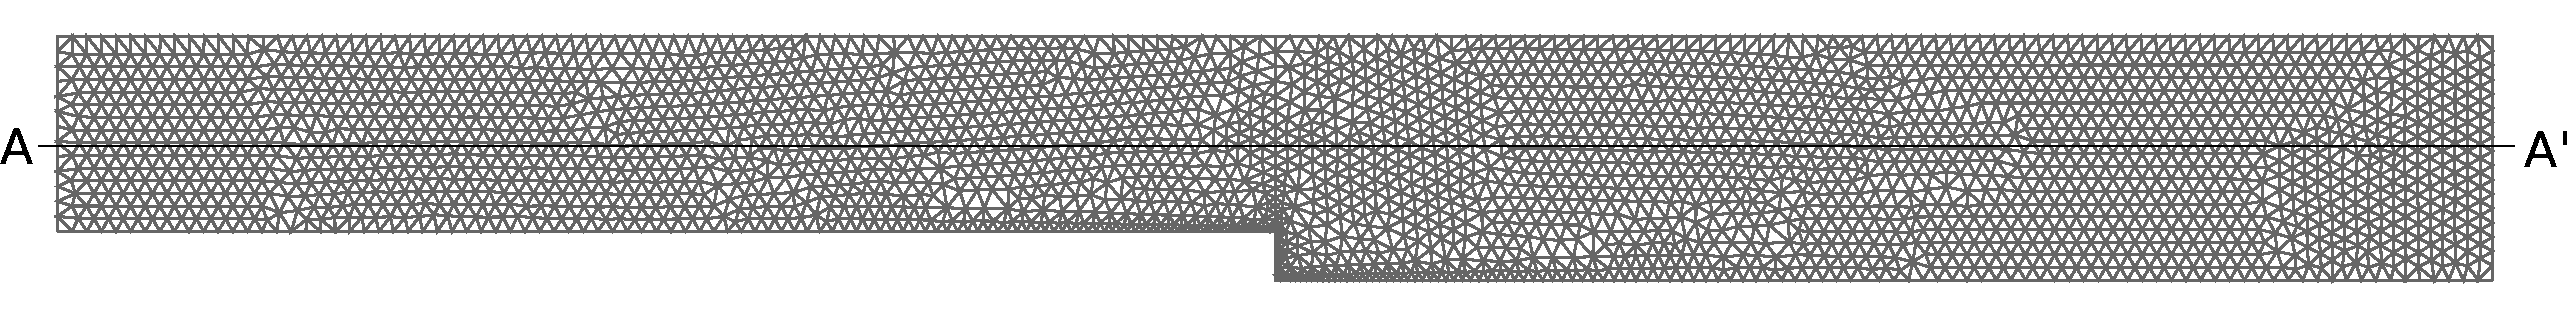
\includegraphics[width=\textwidth]{img/step/mesh.pdf}
    \caption{Channel with a backward step. Domain and mesh used in the simulation. The average element size is $0.06m$. Near the obstacle the mesh size is $0.02m$. There are $3.125$ nodes and $5.826$ elements.}
    \label{step_mesh}
\end{figure}

\begin{figure}[H]
\begin{subfigure}{\textwidth}
    \centering
    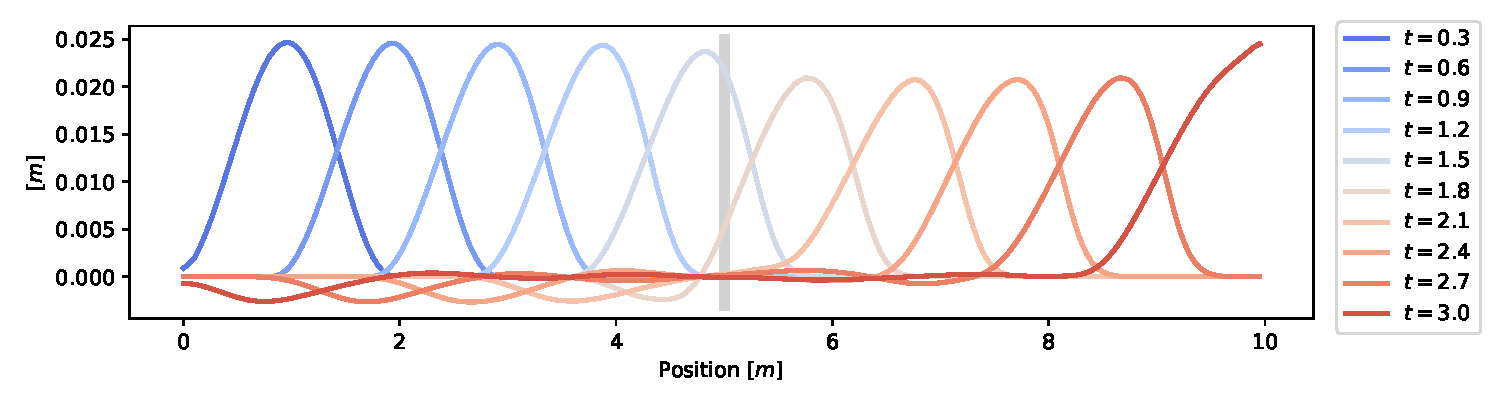
\includegraphics[width=\textwidth]{img/step/free_surface_1.pdf}
    \caption{Time from $0$ to $3s$}
\end{subfigure}
\begin{subfigure}{\textwidth}
    \centering
    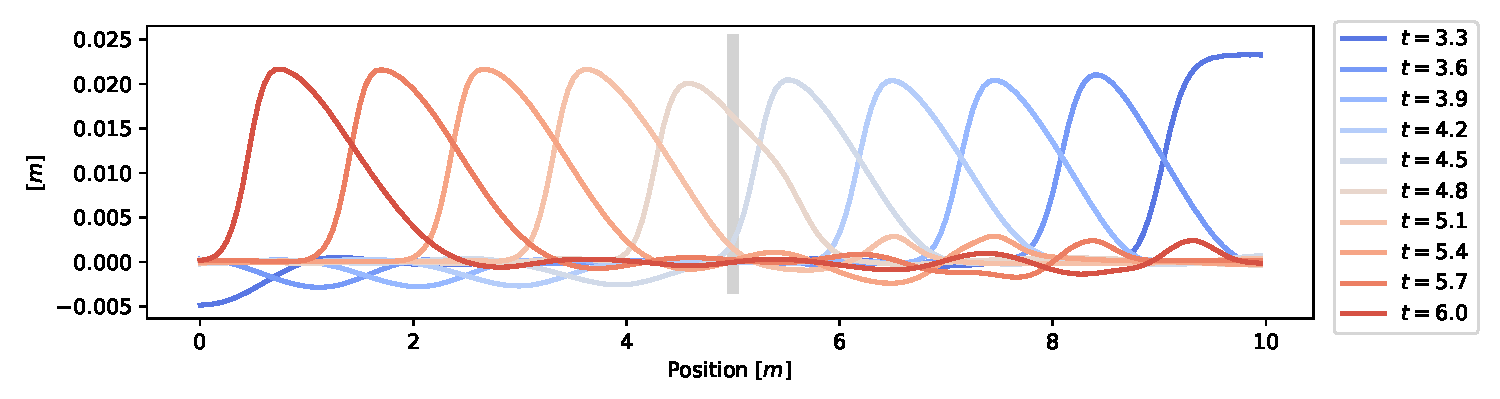
\includegraphics[width=\textwidth]{img/step/free_surface_2.pdf}
    \caption{Time from $3$ to $6s$}
\end{subfigure}
\caption{Channel with a backward step. Timestamps of the free surface along the cut AA' from Figure \ref{step_mesh}. (a) The initial perturbation is propagating to the right. (b) Propagation of the reflected wave from right to left.}
\label{waves_propagation}
\end{figure}


The best results are achieved with the intermediate value and it has been fixed for the rest of the examples in this paper.
Figures \ref{stab_parameters_time1} and \ref{stab_parameters_time2} show that the lower value of $\beta$ is not enough to provide stability, while the higher value is over diffusive.

\begin{figure}[H]
\begin{subfigure}{.05\textwidth}
    \caption{}
\end{subfigure}
\begin{minipage}[c]{.94\textwidth}
    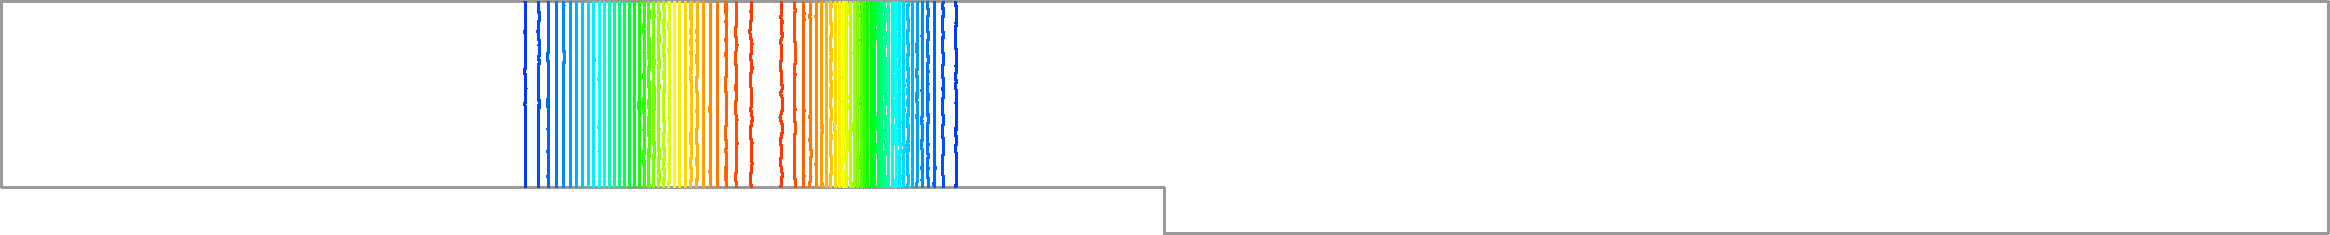
\includegraphics[width=\textwidth]{img/step/stab_0.001_time_1.pdf}        
\end{minipage}
\par\medskip
\begin{subfigure}{.05\textwidth}
    \caption{}
\end{subfigure}
\begin{minipage}[c]{.94\textwidth}
    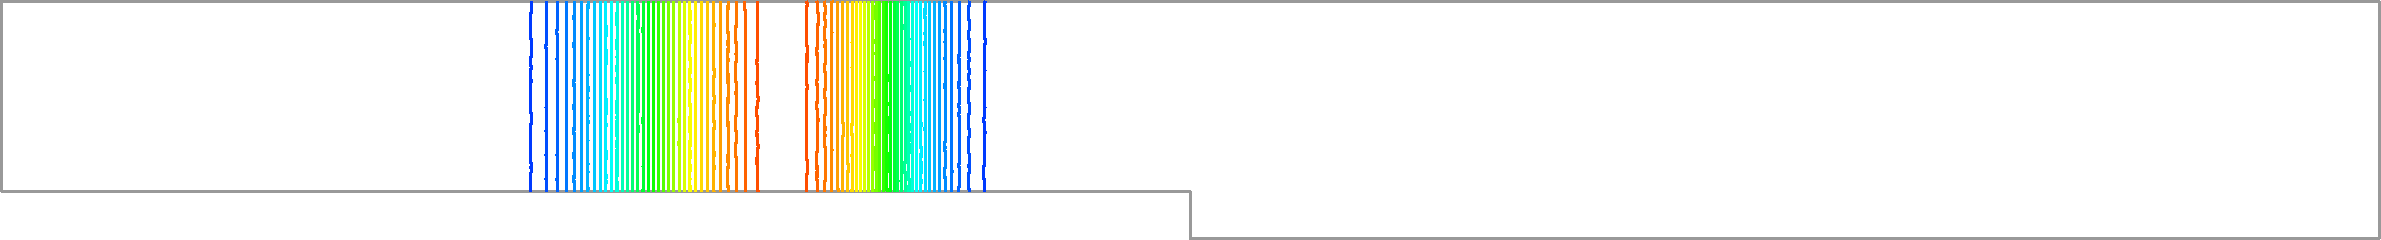
\includegraphics[width=\textwidth]{img/step/stab_0.01_time_1.pdf}        
\end{minipage}
\par\medskip
\begin{subfigure}{.05\textwidth}
    \caption{}
\end{subfigure}
\begin{minipage}[c]{.94\textwidth}
    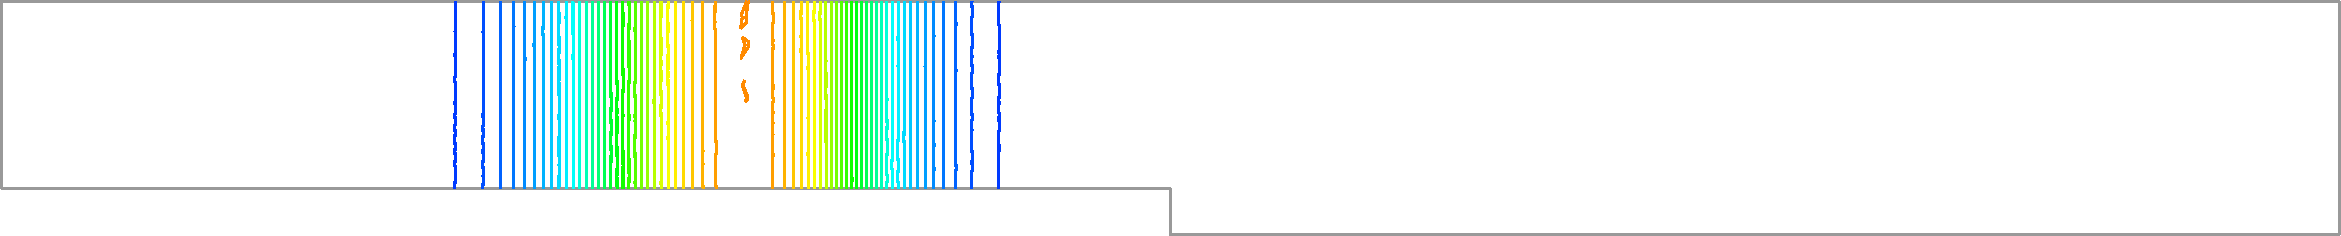
\includegraphics[width=\textwidth]{img/step/stab_0.1_time_1.pdf}        
\end{minipage}
\caption{Channel with a backward step. Contour plots of the free surface elevation at time $t=1s$ for different stabilization factors. (a) $\beta=0.001$, (b) $\beta=0.01$, (c) $\beta=0.1$}
\label{stab_parameters_time1}
\end{figure}

\begin{figure}[H]
    \begin{subfigure}{.05\textwidth}
        \caption{}
    \end{subfigure}
    \begin{minipage}[c]{.94\textwidth}
        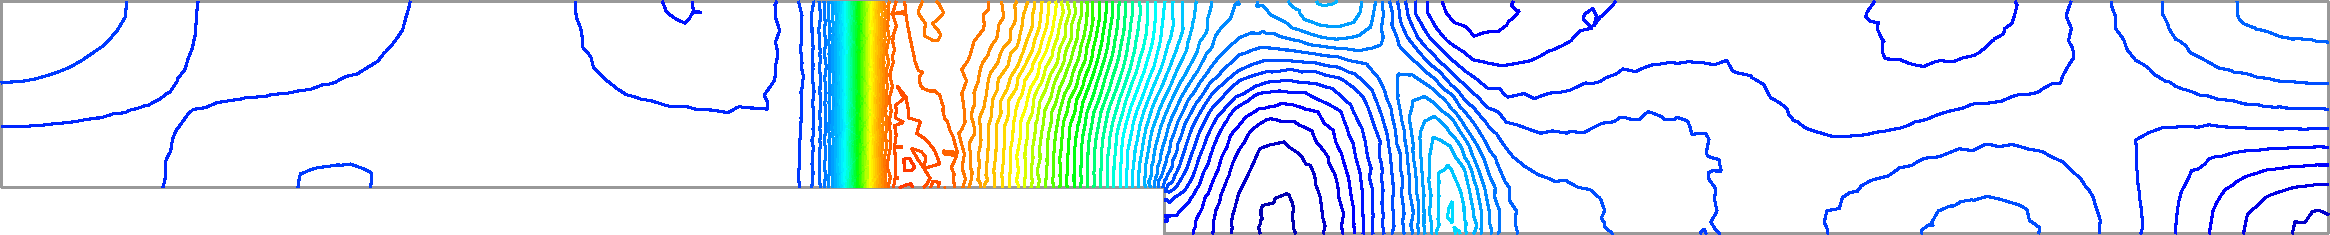
\includegraphics[width=\textwidth]{img/step/stab_0.001_time_5.pdf}
    \end{minipage}
    \par\medskip
    \begin{subfigure}{.05\textwidth}
        \caption{}
    \end{subfigure}
    \begin{minipage}[c]{.94\textwidth}
        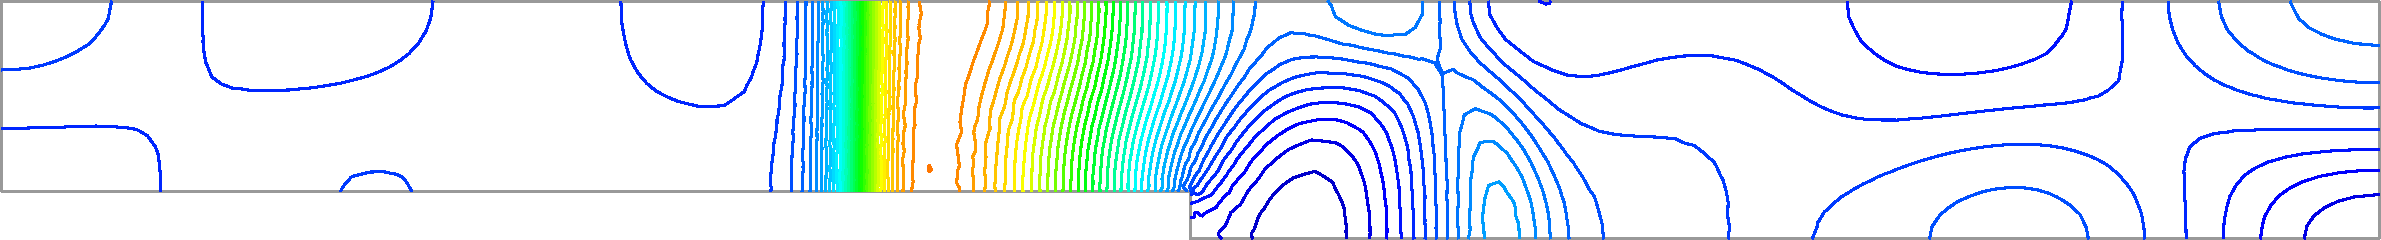
\includegraphics[width=\textwidth]{img/step/stab_0.01_time_5.pdf}
    \end{minipage}
    \par\medskip
    \begin{subfigure}{.05\textwidth}
        \caption{}
    \end{subfigure}
    \begin{minipage}[c]{.94\textwidth}
        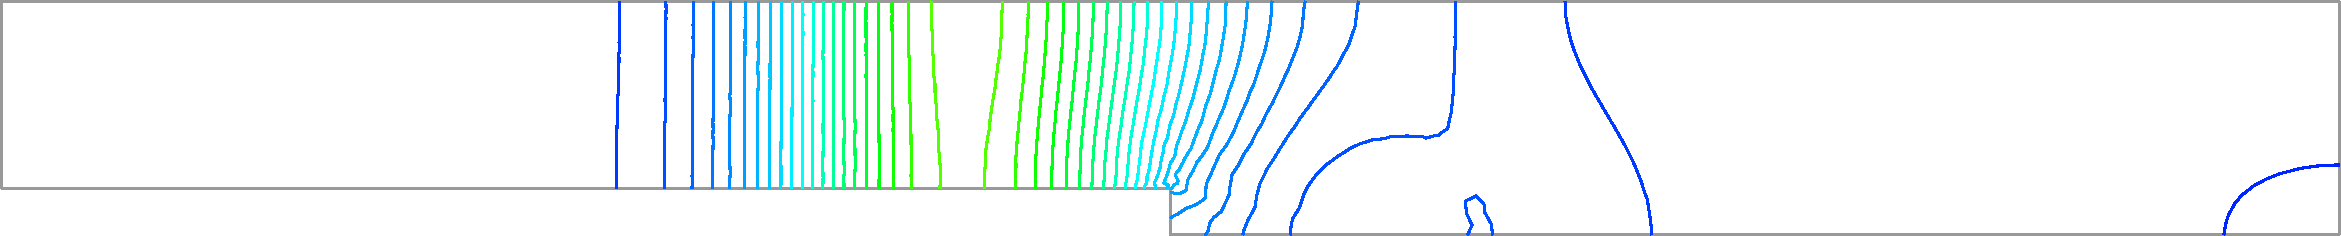
\includegraphics[width=\textwidth]{img/step/stab_0.1_time_5.pdf}
    \end{minipage}
\caption{Channel with a backward step. Contour plots of the free surface elevation at time $t=5s$ for different stabilization factors. (a) $\beta=0.001$, (b) $\beta=0.01$, (c) $\beta=0.1$}
\label{stab_parameters_time2}
\end{figure}



\subsection{Oscillation in a parabolic basin}

The second example is a classical benchmark oriented to test the accuracy of the location of the moving boundary. The topography follows a parabolic profile while the initial free surface elevation is planar and intersects the topography. The initial configuration corresponds to water at rest but the free surface is in a non horizontal plane. The solution of the problem is an oscillation where the free surface elevation remains planar. An analytical solution can be found in the compilation made by Delestre et al. \cite{delestre2013}.

The domain $\Omega$ is defined in the interval $[0,L]\times[0,1]m$ where $L=10$ and all the boundaries are reflective ($\mathbf{u}\cdot\mathbf{n} = 0$). The topography is given by the following expression
\begin{equation}
z(x,y) = h_0 \left(\frac{1}{a^2}\left(x - \frac{L}{2}\right)^2 - 1\right)
\end{equation}
The primitive variables are defined by
\begin{subequations}
\begin{align}
h(x,y) &=
\begin{cases}
-h_0\left(\left(\frac{1}{a}\left(x - \frac{L}{2}\right) + \frac{1}{2a}\cos(2Bt)\right)^2 - 1\right)
\quad &\text{if} \ x_1(t) < x < x_2(t) \\
0 \quad &\text{otherwise}
\end{cases} \\
\mathbf{u}(x,y) &=
\begin{cases}
(B,0)\sin(2Bt) \quad &\text{if} \ x_1(t) < x < x_2(t) \\
(0,0) \quad &\text{otherwise}
\end{cases}
\end{align}
\end{subequations}
where $B=\sqrt{2gh_0}/2a$, and $x_1$, $x_2$ are time dependent functions which define the location of the dry-wet interface:
\begin{equation}
\begin{split}
x_1(t) = -\frac{1}{2}\cos(2Bt) - a + \frac{L}{2} \\
x_2(t) = -\frac{1}{2}\cos(2Bt) + a + \frac{L}{2}
\end{split}
\end{equation}

The domain $\Omega$ is discretized using several meshes in order to perform a convergence analysis. The meshes employed are listed in Table \ref{parabola_convergence}. Figure \ref{parabola_mesh} shows one of the intermediate mesh. Once the simulation begins, the water starts to oscillate on the parabolic basin and the velocity field is constant on the spatial domain, while follows a periodic function respect the time. Figure \ref{parabola_graphic} shows a cut along the mesh. The most challenging problem is to capture the discontinuity of the velocity. Even though the velocity presents a discontinuity, the shock capturing is not required, since it is not a degree of freedom.

Figure \ref{parabola_results} show the results using the finest mesh. The discretization is not shown for the sake of simplicity. As expected, there is no variation on the results in the transversal section.

\begin{figure}
    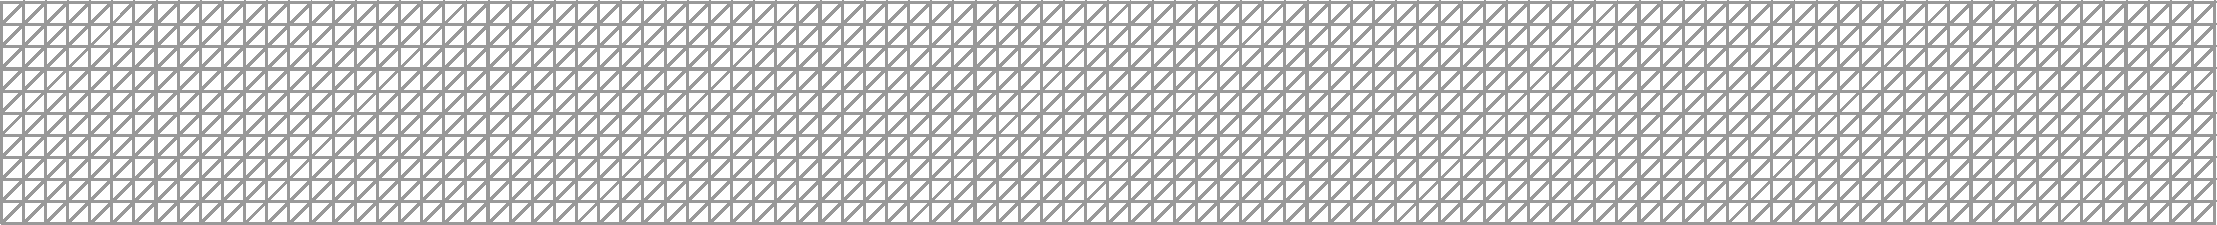
\includegraphics[width=\textwidth]{img/par/mesh_0.1.pdf}
    \caption{Parabolic basin. One of the meshes used in the analysis. The element size is $0.1m$.}
    \label{parabola_mesh}
\end{figure}

\begin{figure}[H]
\begin{subfigure}{0.4\textwidth}
    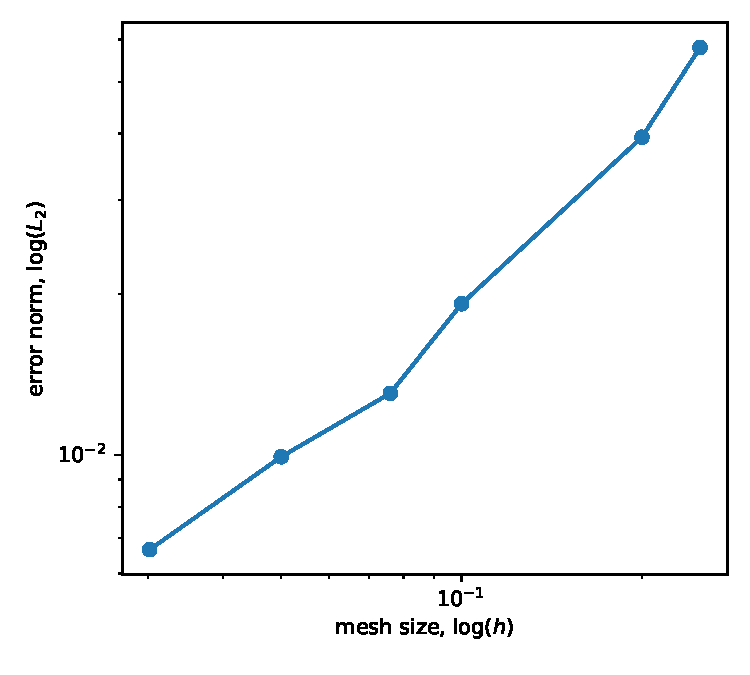
\includegraphics[width=\textwidth]{img/par/conv_1.pdf}    
\end{subfigure}
\hfill
\begin{subfigure}{0.58\textwidth}
    \begin{tabular}{>{\small}rcccc} \hline
    $n_{nodes}$ & $\Delta x$ & $\Delta t$ & CFL & $L_2(e_{rel})$ \\ \hline
205 & 0.25 & 0.008 & 0.5 & 0.24 \\
1,111 & 0.1 & 0.003 & 0.5 & 0.064 \\
4,221 & 0.05 & 0.002 & 0.5 & 0.023 \\
11,356 & 0.03 & 0.001 & 0.5 & 0.013 \\
101,101 & 0.01 & 0.0003 & 0.5 & 0.0049 \\
    \hline
    \end{tabular}
\end{subfigure}
\caption{Parabolic basin. Convergence analysis for the water height.}
\label{parabola_convergence}
\end{figure}

\begin{figure}[H]
\begin{subfigure}{\textwidth}
    \centering
    Time $t=0.5s$
    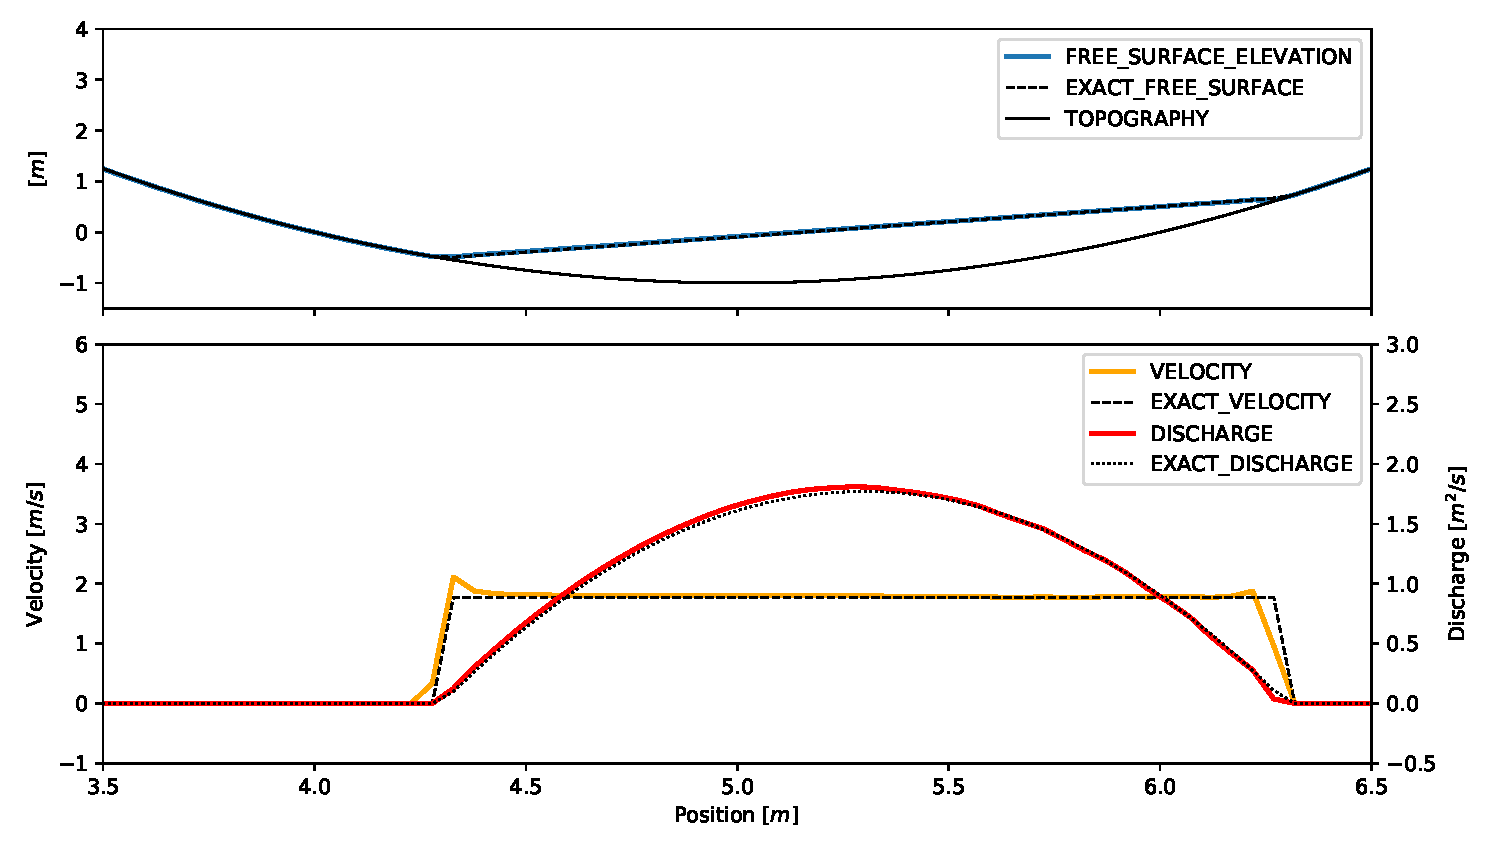
\includegraphics[width=\textwidth]{img/par/parabola_t0.5.pdf}
\end{subfigure}
\par\medskip
\begin{subfigure}{\textwidth}
    \centering
    Time $t=1s$
    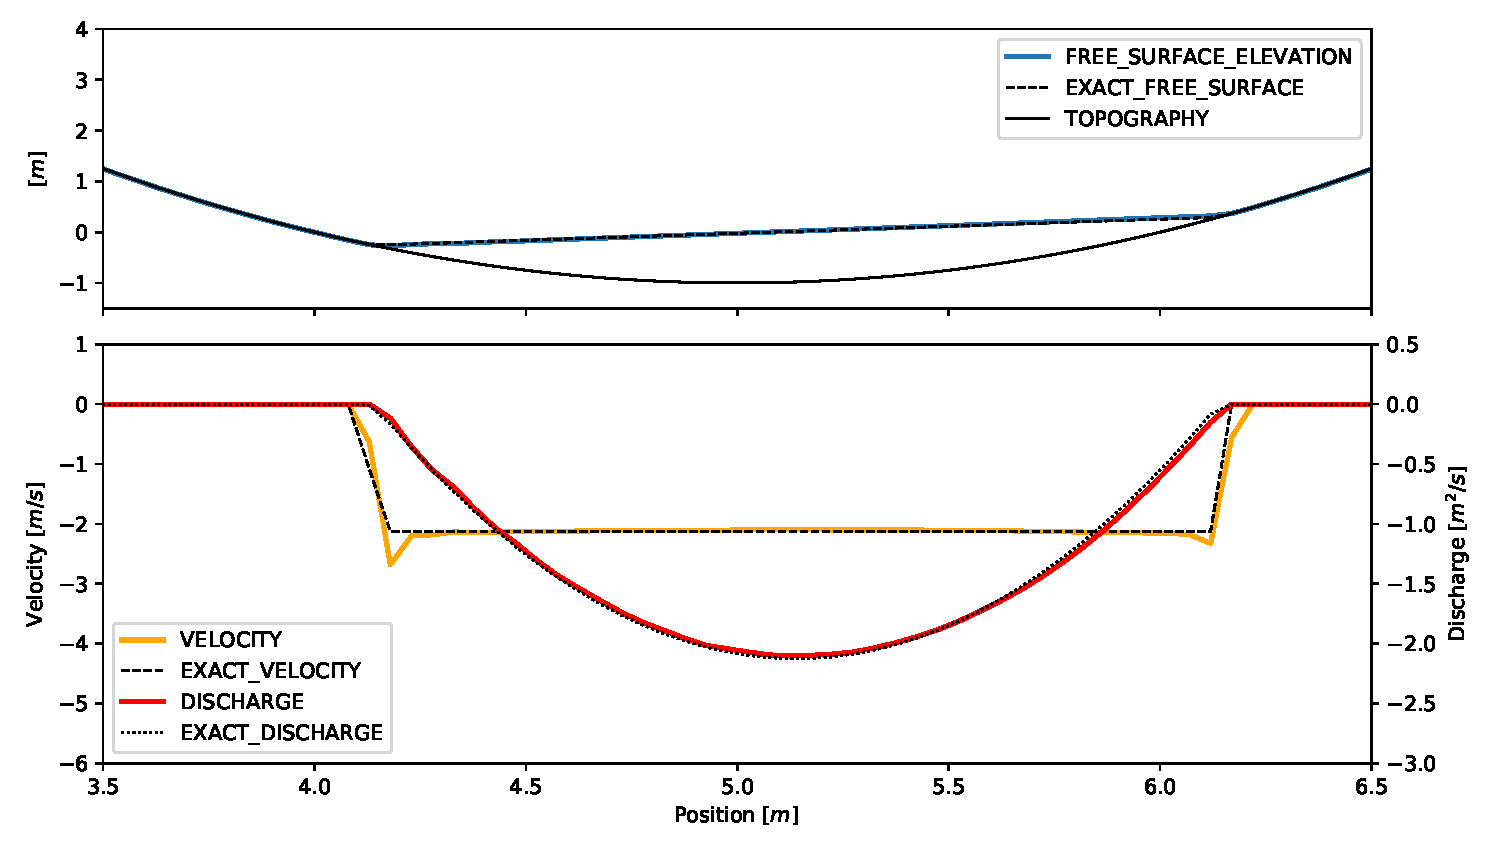
\includegraphics[width=\textwidth]{img/par/parabola_t1.0.pdf}
\end{subfigure}
\caption{Parabolic basin. Cuts along the mesh of size $0.03m$ at different times. There are 333 nodes on the cut.}
\label{parabola_graphic}
\end{figure}

\begin{figure}[H]
    \begin{subfigure}{.05\textwidth}
        \caption{}
    \end{subfigure}
    \begin{minipage}[c]{.94\textwidth}
        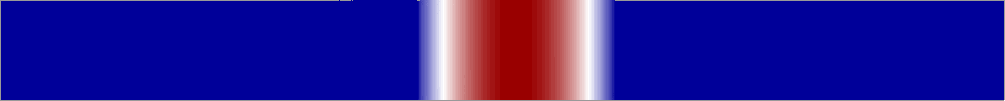
\includegraphics[width=\textwidth]{img/par/height_1.0.png}
    \end{minipage}
\par\medskip
    \begin{subfigure}{.05\textwidth}
        \caption{}
    \end{subfigure}
    \begin{minipage}[c]{.94\textwidth}
        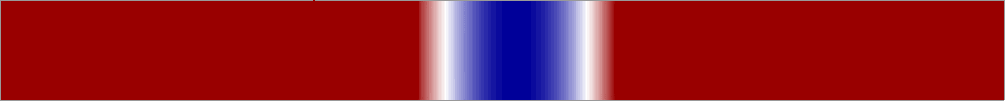
\includegraphics[width=\textwidth]{img/par/momentum_1.0.png}
    \end{minipage}
\par\medskip
    \begin{subfigure}{.05\textwidth}
        \caption{}
    \end{subfigure}
    \begin{minipage}[c]{.94\textwidth}
        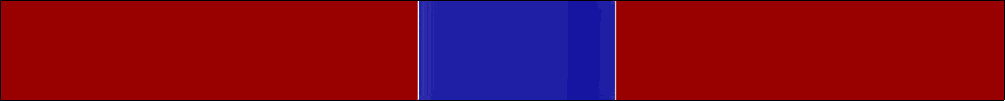
\includegraphics[width=\textwidth]{img/par/velocity_1.0.png}
    \end{minipage}
\caption{Parabolic basin. Results with the fine mesh of size $0.01m$ at time $t=1s$. (a) Water height, (b) x-discharge and (c) x-velocity. There is no legend for simplicity, the red colour is positive and blue means a null or negative magnitude.}
\label{parabola_results}
\end{figure}



\subsection{Short channel with smooth transition and shock}

The third example in a benchmark based on the Mac Donald's type solutions \cite{macdonald1997}. The analytical solution can be found in the same compilation than the previous example \cite{delestre2013}. This test presents a channel with a steady state solution. There is a subcritical inlet and a transcritical flow is produced. The outlet is also subcritical and then a shock is generated at $\sfrac{2}{3}$ of the channel. The aim of this example is to evaluate the shock capturing technique presented and the correct location of the hydraulic jump, which depends on the bottom friction law.

Here we will consider the 1D shallow water equations without diffusion and only with Manning bottom friction as source term. A steady state solution satisfies $\pder{q}{x}=0$ and Equation (\ref{general_sw}) reduces to
\begin{equation} \label{steady_state}
\pder{z}{x} = \left(\frac{v^2}{gh}-1\right) \pder{h}{x} - n^2\frac{\abs{v}v}{h^{\sfrac{4}{3}}}
\end{equation}
This relation allows to integrate the topography given an analytical expression for the water height. Another approach in hydraulics is to consider a given discharge and topography and integrate the water height using Equation (\ref{steady_state}). Following both approaches exact solutions can be obtained. Since this expression involves the bottom friction, we can verify if the friction term is correctly coded in order to satisfy the steady state.

For this benchmark we have considered the domain defined by the spatial domain $[0,100]\times[0,5]$ which is a channel of $100m$ length and $5m$ width (Figure \ref{chanel_geometry}), and the following boundary conditions:
\begin{equation}
\begin{split}
    q_x = 2\ \text{m/s} \qquad &\text{in} \ \Gamma_{upstream} \\
    h = h_{ex}(100) \qquad &\text{in} \ \Gamma_{downstream} \\
    q_y = 0 \qquad &\text{in} \ \Gamma_{walls}
\end{split}
\end{equation}
The Manning coefficient is $0.0328\ \text{m}^{-1/3}\text{s}$ and the water height $h_{ex}(x)$ is a piecewise function defined in \cite{delestre2013}. The discontinuity of the water height function is located at $x=200/3\ m$ and defines the hydraulic jump. The expression of the exact water depth is:
\begin{equation} \label{jump_height_definition}
    h = \begin{cases}
        \left(\frac{4}{g}\right)^\frac{1}{3} \left(\frac{4}{3} - \frac{x}{L}\right) - \frac{9x}{10L}
            \left(\frac{x}{L} - \frac{2}{3}\right) \, ,\ \text{for} \ x < \frac{2L}{3}\\
        \left(\frac{4}{g}\right)^\frac{1}{3} \left(
              a_1 \left(\frac{x}{L} - \frac{2}{3}\right)^4
            + a_1 \left(\frac{x}{L} - \frac{2}{3}\right)^3
            - a_2 \left(\frac{x}{L} - \frac{2}{3}\right)^2 \right. \\ \left. \qquad\qquad\qquad\qquad
            + a_3 \left(\frac{x}{L} - \frac{2}{3}\right)
            + a_4
        \right) \, ,\ \text{for} \ x \geq \frac{2L}{3}
    \end{cases}
\end{equation}
where $a_1=0.674202$, $a_2=21.7112$, $a_3=14.492$ and $a_4=1.4305$. The topography is obtained by a numerical integration using the fourth order Runge Kutta method.

As in the previous example, several meshes are employed and a convergence analysis is performed (Figure \ref{hydraulic_jump_convergence}). The shock capturing parameter is $\alpha=1.0$ and we will study the accuracy of the hydraulic jump. 
Given the initial conditions, the hydraulic jump is generated between the first $50$ and $80s$. The overall error is computed at time $t=200s$, in order to ensure the stationary state is achieved.
The table from Figure \ref{hydraulic_jump_convergence} shows the error of the $x$-discharge over all the domain using the $L_2$ norm.

Results from different meshes are compared in Figures \ref{mac_donald_shock_graph_5} and \ref{mac_donald_shock_graph_2}. The oscillations are reduced with the finer mesh (Figure \ref{mac_donald_shock_graph_2}), but there is a peak on the discharge at the location of the shock. This peak is originated because the momentum balance includes the gradient of the total water depth, and the analytical gradient is a Dirac delta function.

\begin{figure}
    
\includegraphics[width=\textwidth]{img/jump/sketch/sketch.pdf}
    \caption{Short channel. Geometry of the channel. The vertical line shows the position of the hydraulic jump.}
    \label{chanel_geometry}
\end{figure}


\begin{figure}
\begin{subfigure}{0.4\textwidth}
    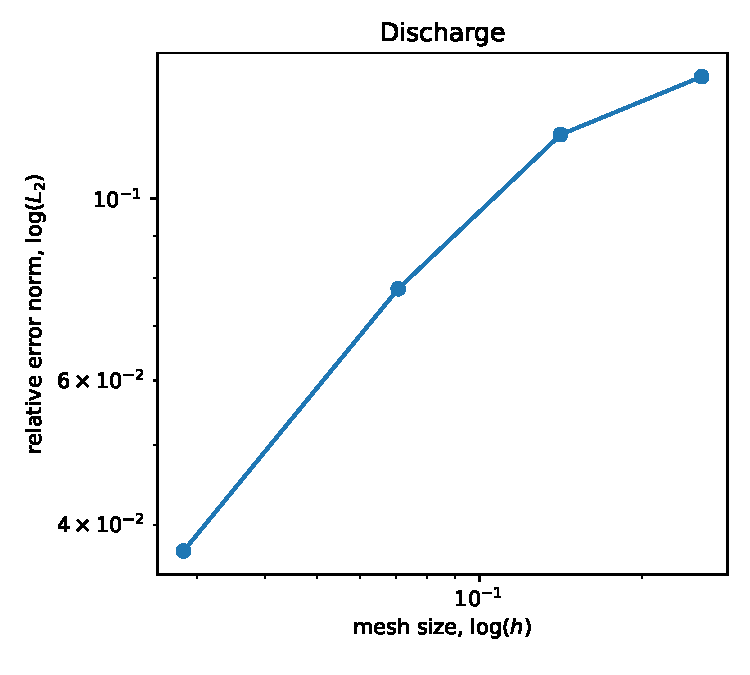
\includegraphics[width=\textwidth]{img/jump/momentum_convergence.pdf}    
\end{subfigure}
\hfill
\begin{subfigure}{0.58\textwidth}
    \begin{tabular}{>{\small}rcccc} \hline
    $n_{nodes}$ & $\Delta x$ & $\Delta t$ & CFL   & $L_2(e_{rel})$ \\ \hline
    204         &        2.0 &      0.005 & 0.016 & 0.177 \\
    606         &        1.0 &      0.005 & 0.031 & 0.138 \\
    2211        &        0.5 &      0.005 & 0.062 & 0.088 \\
    13026       &        0.2 &      0.005 & 0.15  & 0.041 \\ \hline
    \end{tabular}
\end{subfigure}
\caption{Short channel. Convergence analysis for the $x$-discharge.}
\label{hydraulic_jump_convergence}
\end{figure}


\begin{figure}
    \centering
    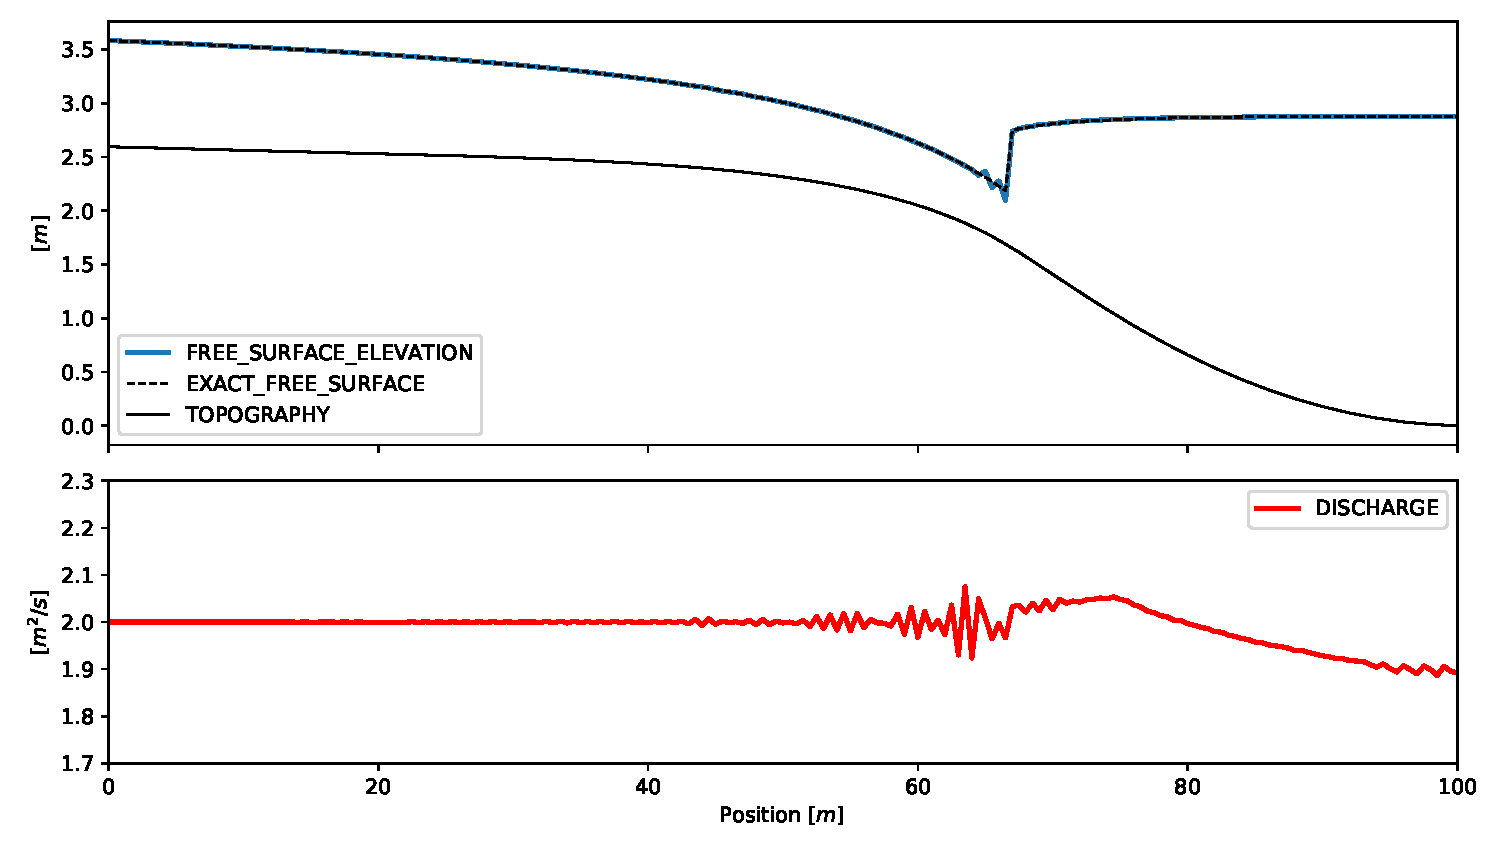
\includegraphics[width=\textwidth]{img/jump/mesh_0.5.pdf}
    \caption{Short channel. Graph along the cut defined by the center of the channel. The mesh size is $0.5m$}
    \label{mac_donald_shock_graph_5}
\end{figure}

\begin{figure}
    \centering
    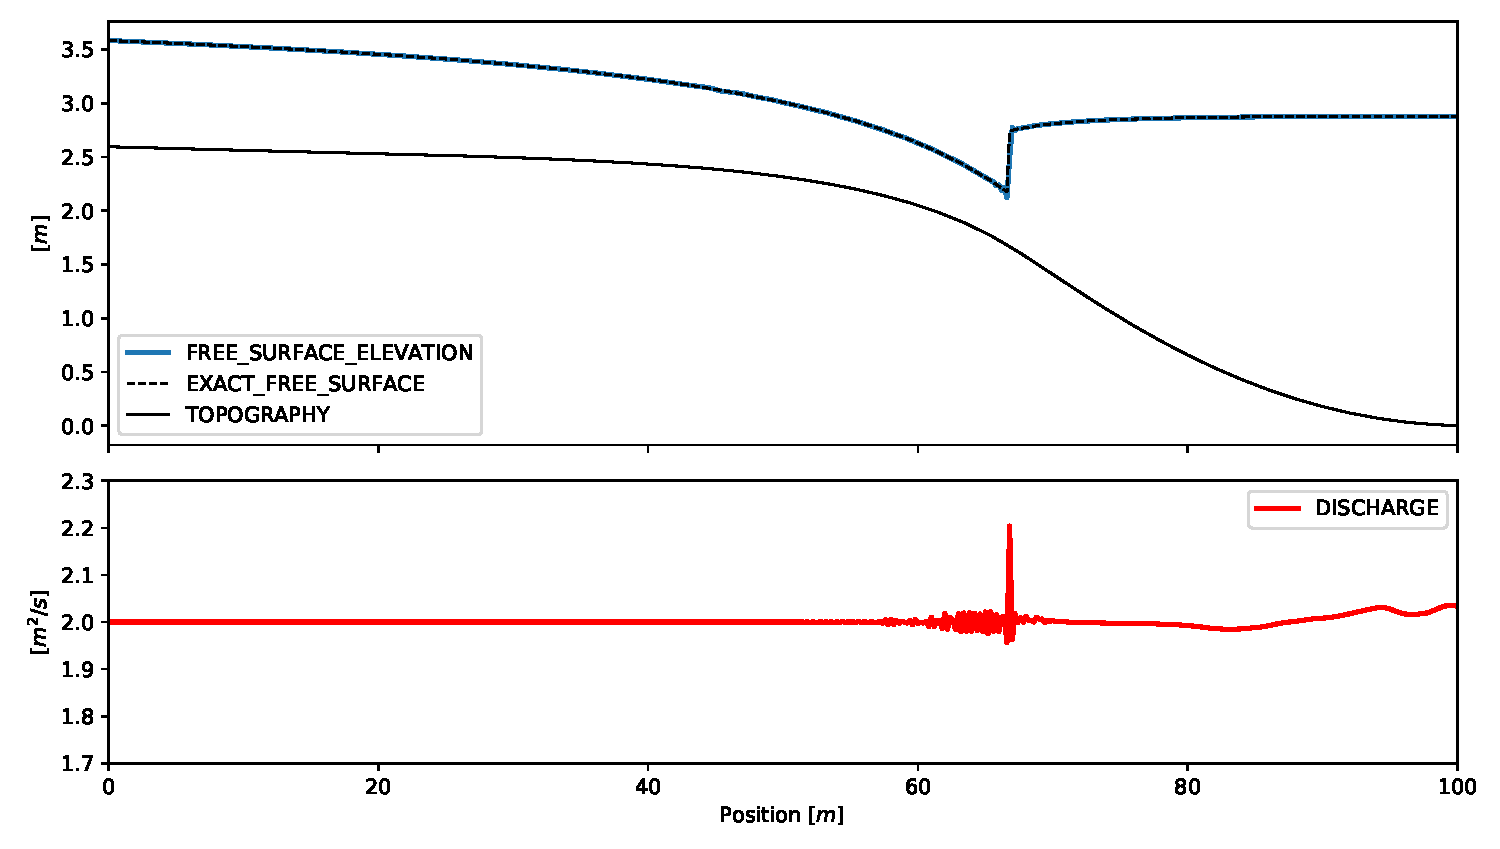
\includegraphics[width=\textwidth]{img/jump/mesh_0.2.pdf}
    \caption{Short channel. Graph along the cut defined by the center of the channel. The mesh size is $0.2m$}
    \label{mac_donald_shock_graph_2}
\end{figure}


\subsection{Experimental dam break flow against an isolated building}

The last example consists on the reproduction of the experiment carried out by Soares \cite{soares2007}.
A dam break flow with a building downstream is simulated. The problem definition is depicted in Figure \ref{experiment_sketch}. The channel is $3.4m$ width and the end of the dam is located at $x=0$.
As initial conditions, the water depth is set to $0.4m$ in the reservoir, while the channel is dry. The Manning coefficient is $0.01ms^{-1}$ over all the domain.
At the beginning of the simulation, the gate of the dam is removed and the water is allowed to flow around the building.
There are some gauges (Table \ref{gauges_positions}) where the water height is recorded and experimental data is used to validate the numerical method.

The domain is discretized with a mesh with an average element size of $0.05m$. There are 115.000 elements and the time step is computed to keep a courant number of 1.0. Figure \ref{experiment_mesh} displays two details of the mesh, near the dam and around the building.

Figure \ref{experiment_plots} shows several results of the water depth after the gate release. Figure \ref{experiment_gauges} shows the evolution of the water depth at the gauges. An initial delay is observed in the propagation of the front in the gauges 1 to 5.
The gauges 1 and 2 show a rise of the water level after the first front is arrived, this behavior correspond to the hydraulic jump generated in front of the building.
Regarding the performance of the FIC-FEM formulation, it captures the main aspects of the flow, but not the details, since there are some regions on that experiment which violate the shallow water approximations.

\begin{figure}[H]
\centering
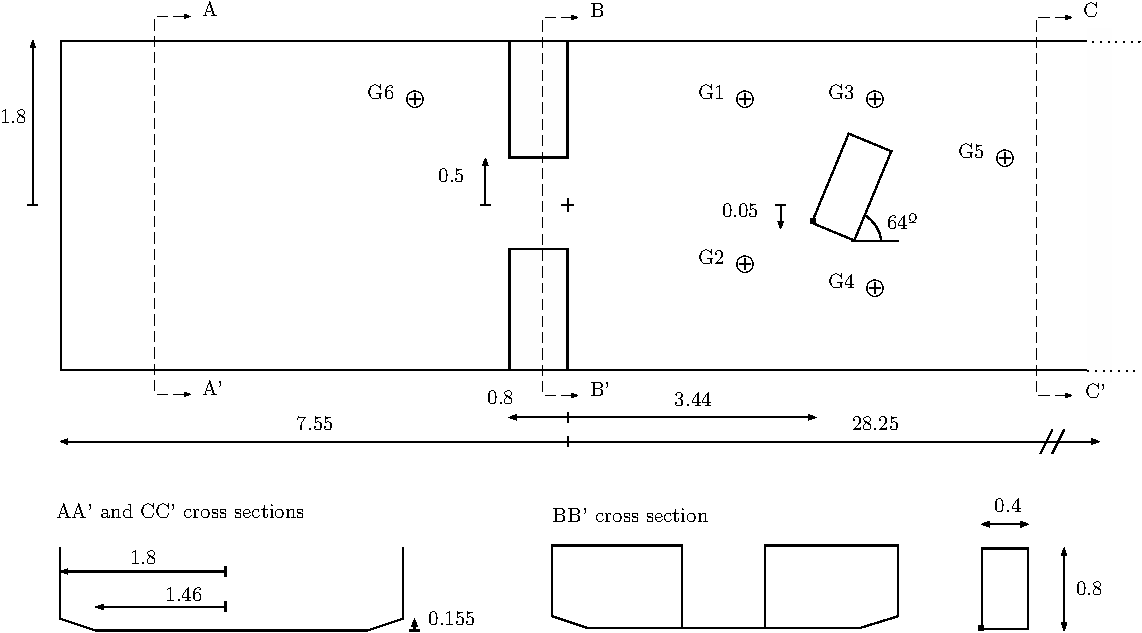
\includegraphics[width=\textwidth]{img/exp/sketch.pdf}
\caption{Experimental dam break flow. Definition of the isolated building benchmark. The dimensions are in $m$.}
\label{experiment_sketch}
\end{figure}


\begin{figure}[H]
\centering
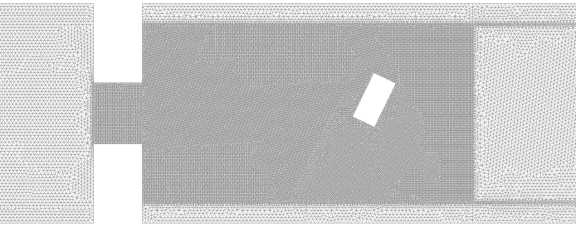
\includegraphics[width=.8\textwidth]{img/exp/experiment_mesh.png}
\caption{Experimental dam break flow. Detail of the mesh near the dam and around the building. The coarse elements have an average size of $0.06m$ and the refined area has an average element size of $0.02m$. There are 160.000 elements.}
\label{experiment_mesh}
\end{figure}


\begin{table}
\centering
\begin{tabular}{ccc}
\hline
Gauge number & X & Y \\ \hline
1 &  2.65 &  1.15 \\
2 &  2.65 & -0.60 \\
3 &  4.00 &  1.15 \\
4 &  4.00 & -0.80 \\
5 &  5.20 &  0.30 \\
6 & -1.87 &  1.10 \\ \hline
\end{tabular}
\caption{Experimental dam break flow. Positions of the gauges, units in $m$.}
\label{gauges_positions}
\end{table}


\begin{figure}
\centering
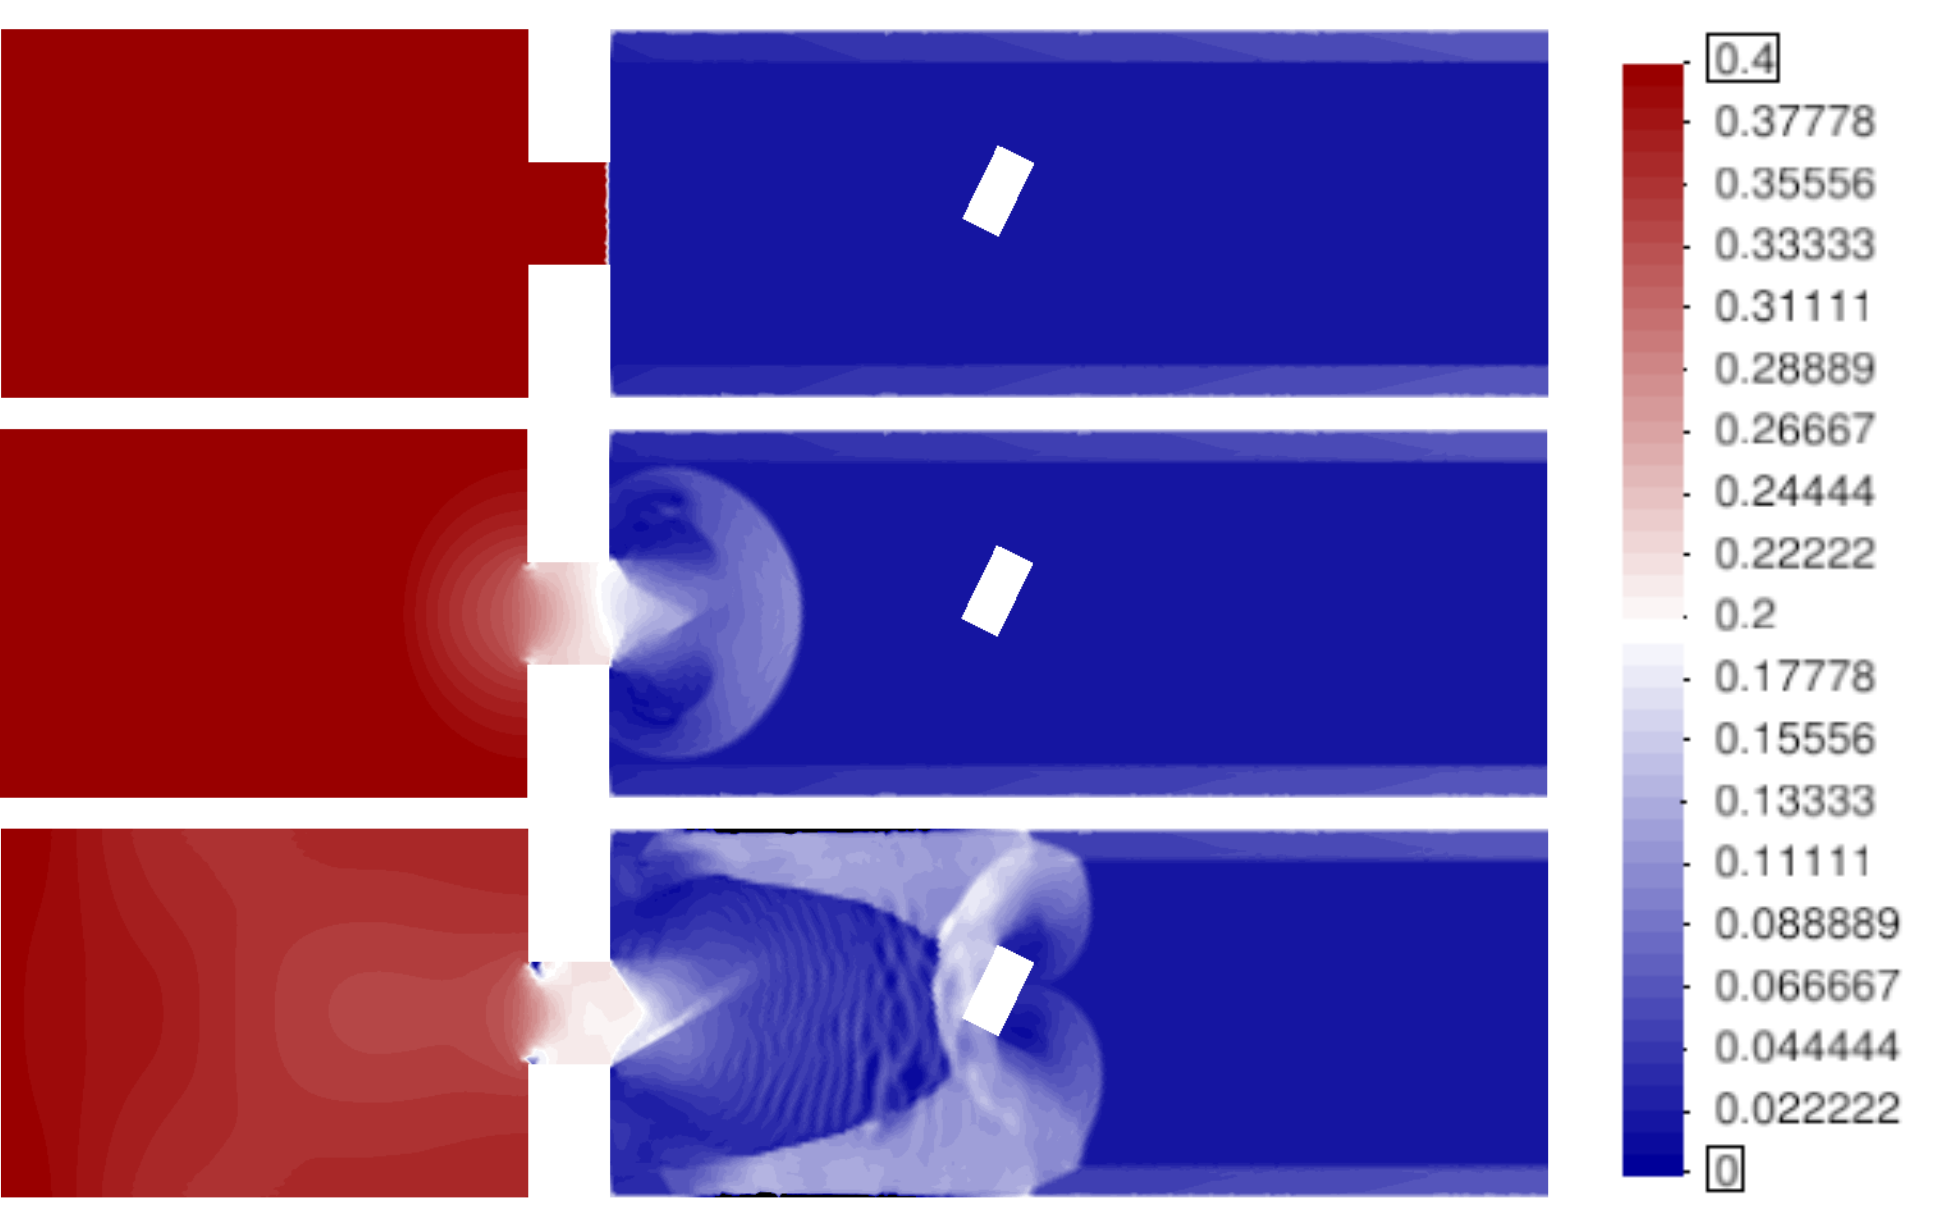
\includegraphics[width=\textwidth]{img/exp/results.png}
\caption{Experimental dam break flow. Results of the benchmark at times $0$, $1$ and $3$ seconds}
\label{experiment_plots}
\end{figure}


\begin{figure}
\centering
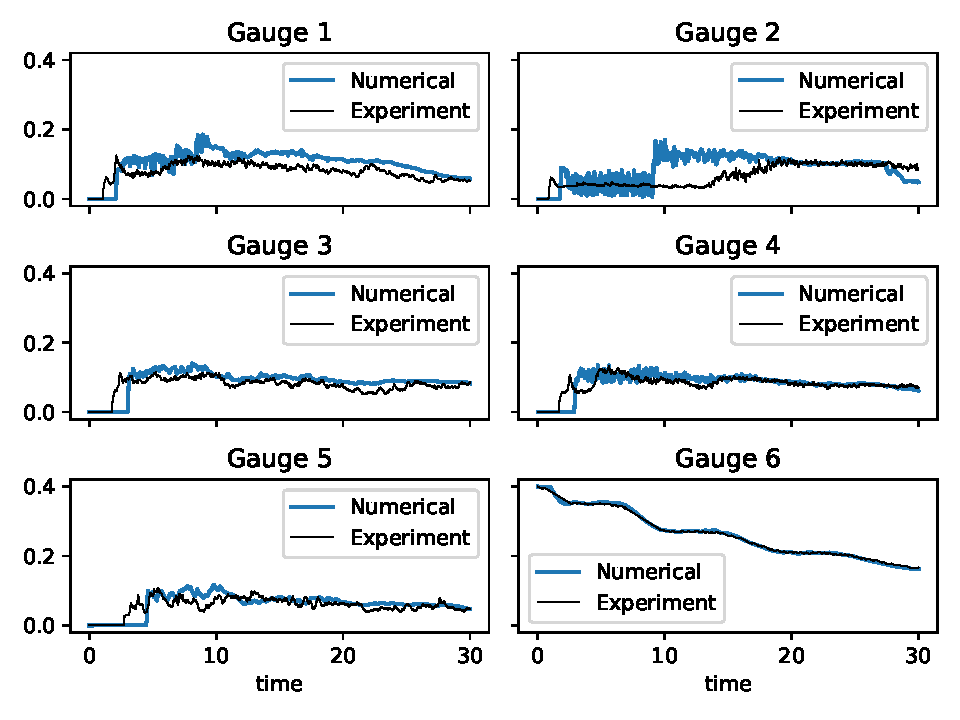
\includegraphics[width=\textwidth]{img/exp/gauges.pdf}
\caption{Experimental dam break flow. Comparison between the obtained water depth with the reference data.}
\label{experiment_gauges}
\end{figure}



\section{Concluding remarks} \label{sec:conclusions}

We have extended the FIC-FEM procedure to the shallow water equations. Unlike the FIC-based stabilizations for incompressible flows, the present procedure is applied to the coupled mass and momentum balance at the same time using the linearization matrix $\mathbf{A}_i$. It can be seen that this procedure casts to the classical FIC-stabilization for convection diffusion problems, taking the velocity as linearization term. The same procedure can be applied to develop stabilized formulations for compressible flows.

The present extension of the FIC-procedure to the shallow water equations uses the linearization matrix $\mathbf{A}_i$ for the flux terms to project the characteristic length. However, an alternative framework can be explored with the ASGS \cite{hughes1995,codina2008} formulation, which includes the linearization matrices of the viscous terms and reaction terms. Since the shallow water equations are dominated by the convective matrix $\mathbf{A}_i$, and thus are strictly hyperbolic, the present stabilization is enough to provide stability, as shown in Section \ref{sec:examples}.

The present stabilization provides two algorithmic constants, one for the global stabilization and other one for the shock capturing term. From our numerical experiments, we have chosen $\beta=0.01$ for the stabilization and $\alpha=1.0$ for the shock capturing.

The present FIC-FEM procedure has produced accurate results for the examples considered.
In the first example, the artificial diffusion is evaluated and it has been proved to be small and practically inappreciable. The shock capturing term allows to solve supercritical problems with discontinuities and the present procedure is also able to deal with partially wet domains. Finally, a numerical simulation of a dam break flow against an isolated building is performed showing a good agreement with the experimental data.



\section{Acknowledgements}

The first author gratefully acknowledges the Universitat Politècnica de Catalunya and Banco Santander for the financial support for his pre-doctoral grant (53 FPI-UPC 2018).
This research was partially funded by the project PARAFLUIDS (PID2019-104528RB-I00). The authors also acknowledge the financial support from the CERCA programme of the Generalitat de Catalunya, Spain, and from the Spanish Ministry of Economy and Competitiveness, through the “Severo Ochoa Programme for Centres of Excellence in R\&D”, Spain (CEX2018-000797-S).



\section*{Appendix A}
\addcontentsline{toc}{section}{Appendix A}

The stabilization matrices are the result of multiplying $\mathbf{A}$ tensor by itself:

\begin{subequations}
\begin{equation}
\mathbf{A}_1\mathbf{A}_1 =
\begin{pmatrix}
3u_1^2 + c^2 & 0  & -2u_1^3 + 2u_1c^2 \\
2u_1u_2  & u_1^2  & -2u_1^2u_2 + u_2c^2 \\
2u_1  & 0   & -u_1^2 + c^2
\end{pmatrix}
\end{equation}
\begin{equation}
    \mathbf{A}_2\mathbf{A}_2 =
\begin{pmatrix}
u_2^2  & 2u_1u_2  & -2u_1u_2^2 + u_1c^2 \\
0    & 3u_2^2 + c^2 & -2u_2^3 + 2u_2c^2 \\
0  & 2u_2  & -u_2^2 + c^2
\end{pmatrix}
\end{equation}
\begin{equation}
\mathbf{A}_1\mathbf{A}_2 =
\begin{pmatrix}
2u_1u_2  & u_1^2 + c^2  & -2u_1^2u_2 \\
u_2^2  & 2u_1u_2  & -2u_1u_2^2 + u_1c^2 \\
u_2  & u_1  & -u_1u_2
\end{pmatrix}
\end{equation}
\begin{equation}
\mathbf{A}_2\mathbf{A}_1 =
\begin{pmatrix}
2u_1u_2  & u_1^2  & -2u_1^2u_2 + u_2c^2 \\
u_2^2 + c^2  & 2u_1u_2  & -2u_1u_2^2 \\
u_2  & u_1  & -u_1u_2
\end{pmatrix}
\end{equation}
\end{subequations}


\biboptions{sort&compress}
\bibliographystyle{elsarticle-num}
\bibliography{../bibliography/sw}

\end{document}
